\documentclass[10pt,a4paper,oneside]{article}

% ---------------------------------------------------------------------------
% plataforma-mapa-en.tex -- en-US version of `plataforma-mapa.tex`.
%
% PARITY WITH THE PORTUGUESE FILE. This is a translation, not a fork: both
% documents carry the same sections, the same tables, the same numbers and
% the same figures. A change in one belongs in the other.
%
% DELIBERATE DIVERGENCES FROM THE SOURCE FILE:
%
%   `babel` loads `american`. The cover block, the footer and the revision
%   history come from the shared preamble with Portuguese labels; they are
%   redefined below, locally, so the preamble keeps serving the Portuguese
%   documents unchanged.
%
%   Numbers follow en-US: decimal point, comma as thousands separator.
%
%   The two diagrams are the `-en` renderings of `plataforma-mapa-en.puml`.
%
%   Product names are the ones of the interface, which is in English, so the
%   product table carries one name per product instead of two.
%
%   Agency names, dataset names, schema names and regulation numbers stay as
%   in the source: they are identifiers.
%
% Base preamble of the repository: font, type area, packages, caption, title
% and header. Compile from inside `docs/product/`.
% ---------------------------------------------------------------------------
\usepackage[american]{babel}
% =====================================================================
%  Preâmbulo base: pacotes, tipografia e convenções de todo documento
%  LaTeX do repositório
%
%  Origem: `config/preambulo.tex` do documento de projeto do rhae-sensor.
%  As seções abaixo seguem a ordem de lá, e o que difere está marcado
%  com DIFERENÇA.
%
%  Convenções tipográficas e de apresentação adotadas
%    ISO 216        formato A4
%    ISO 80000-1    números e unidades (vírgula decimal, espaço fino entre
%                   grupos de três algarismos, unidade em tipo romano)
%    Tabelas sem filetes verticais (booktabs); legenda de tabela acima,
%    de figura abaixo.
%
%  Uso, antes do `\begin{document}`:
%    report/*.tex          via `\usepackage{estilo-reporte}`, que carrega este
%    docs/product/*.tex    % =====================================================================
%  Preâmbulo base: pacotes, tipografia e convenções de todo documento
%  LaTeX do repositório
%
%  Origem: `config/preambulo.tex` do documento de projeto do rhae-sensor.
%  As seções abaixo seguem a ordem de lá, e o que difere está marcado
%  com DIFERENÇA.
%
%  Convenções tipográficas e de apresentação adotadas
%    ISO 216        formato A4
%    ISO 80000-1    números e unidades (vírgula decimal, espaço fino entre
%                   grupos de três algarismos, unidade em tipo romano)
%    Tabelas sem filetes verticais (booktabs); legenda de tabela acima,
%    de figura abaixo.
%
%  Uso, antes do `\begin{document}`:
%    report/*.tex          via `\usepackage{estilo-reporte}`, que carrega este
%    docs/product/*.tex    % =====================================================================
%  Preâmbulo base: pacotes, tipografia e convenções de todo documento
%  LaTeX do repositório
%
%  Origem: `config/preambulo.tex` do documento de projeto do rhae-sensor.
%  As seções abaixo seguem a ordem de lá, e o que difere está marcado
%  com DIFERENÇA.
%
%  Convenções tipográficas e de apresentação adotadas
%    ISO 216        formato A4
%    ISO 80000-1    números e unidades (vírgula decimal, espaço fino entre
%                   grupos de três algarismos, unidade em tipo romano)
%    Tabelas sem filetes verticais (booktabs); legenda de tabela acima,
%    de figura abaixo.
%
%  Uso, antes do `\begin{document}`:
%    report/*.tex          via `\usepackage{estilo-reporte}`, que carrega este
%    docs/product/*.tex    \input{../../report/config/preambulo}
%
%  FORMA DE MANUAL TÉCNICO. Fonte, números, legendas e pacotes vêm da
%  origem. A forma da página não: é de manual de referência, e não de
%  artigo. Coluna única, títulos recuados para a esquerda do texto,
%  rodapé com identificação e "página X de Y" em toda página, avisos com
%  palavra de sinal (ANSI Z535.6), passos numerados e histórico de
%  revisões (IEC/IEEE 82079-1). O desenho de página segue a classe
%  `refman` do CTAN.
%
%  O documento carrega `babel` ANTES deste arquivo. Documento deitado, que
%  existe para caber tabela larga, carrega também `geometry` antes; aí a
%  margem de manual não entra e os títulos não avançam.
%
%  Motor: pdflatex. Charis SIL, newtxmath e Bera Mono entram como Type 1
%  em T1, e a matemática do newtxmath não passa pelo `unicode-math`.
% =====================================================================
\RequirePackage{iftex}
\RequirePDFTeX
% Este arquivo entra tanto de um `.tex` quanto de dentro do
% `estilo-reporte.sty`, onde o `@` ja e letra. O codigo de categoria e
% devolvido como estava, e nao forcado a "outro" no fim.
\edef\pbrestauraarroba{\catcode`\noexpand\@=\the\catcode`\@\relax}
\makeatletter

% ---------------------------------------------------------------------
%  Fontes, idioma e microtipografia
% ---------------------------------------------------------------------
\usepackage[T1]{fontenc}
\usepackage[utf8]{inputenc}
% DIFERENÇA: o idioma é do documento, porque há documento em inglês.
\@ifpackageloaded{babel}{}{\usepackage[brazilian]{babel}}
\usepackage{CharisSIL}
\usepackage[charter]{newtxmath}
\usepackage[scaled=0.83]{beramono}
\usepackage[protrusion=true,expansion=true,tracking=true]{microtype}
\SetTracking{encoding=*,shape=sc}{40}
% DIFERENÇA: a origem não usa sem serifa. Os documentos daqui pedem
% `\sffamily` em título, tabela e nota; sem esta linha ela cairia na
% Computer Modern Sans, que não pertence ao conjunto. Uma família só.
\renewcommand{\sfdefault}{\rmdefault}

% DIFERENÇA: mancha de manual, e não a coluna de 468 pt da origem. A4 com
% 22 mm de margem de cada lado, 166 mm úteis. O texto corre em 152 mm e
% os 14 mm da esquerda são o recuo dos títulos: o bastante para o título
% sair do alinhamento do texto, sem deixar coluna vazia ao lado dele. A
% primeira versão reservava 40 mm, e a margem ficava em branco em toda
% página que não fosse título; o documento crescia um terço só por isso.
% `\margemmanual` é quanto os títulos, o cabeçalho e o rodapé avançam
% para a esquerda; vale zero quando o documento traz mancha própria.
% A altura é de 253 mm, a mesma da mancha anterior, porque as tabelas
% deitadas foram dimensionadas para ela.
\newlength{\margemmanual}
\@ifpackageloaded{geometry}{\setlength{\margemmanual}{0pt}}{%
  \setlength{\margemmanual}{14mm}%
  \usepackage[a4paper,left=36mm,right=22mm,top=20mm,bottom=24mm,
              headheight=14pt,headsep=7mm,footskip=12mm]{geometry}}

\usepackage{amsmath}
\usepackage[dvipsnames,table]{xcolor}
\usepackage{graphicx}
\usepackage{tikz}
\usepackage{booktabs}
\usepackage{tabularx}
\usepackage{array}
\usepackage{xltabular}
\usepackage{float}
\usepackage{pdflscape}
\usepackage{rotating}
% Página com o conteúdo girado, mas exibida em retrato no leitor de PDF
\newenvironment{paisagemretrato}{\begingroup\def\PLS@AddRotate##1{}\landscape}{\endlandscape\endgroup}
\usepackage{enumitem}
\usepackage{changepage}
\usepackage[most]{tcolorbox}
\usepackage{caption}
\usepackage{titlesec}
\usepackage{fancyhdr}
\usepackage{lastpage}
\usepackage{csquotes}
\usepackage{siunitx}
% DIFERENÇA: sem `biblatex`. Nenhum documento daqui tem `.bib`; as
% referências são listas escritas à mão.
\usepackage{xurl}
\usepackage[hidelinks,pdfusetitle]{hyperref}

% ---------------------------------------------------------------------
%  Números e unidades (ISO 80000-1)
% ---------------------------------------------------------------------
\sisetup{
  output-decimal-marker = {,},
  group-separator       = {\,},
  group-minimum-digits  = 4,
  exponent-product      = \cdot,
  uncertainty-mode      = separate,
  range-phrase          = {\,a\,},
  list-pair-separator   = {\ e\ },
  list-final-separator  = {\ e\ },
  per-mode              = symbol,
}

% ---------------------------------------------------------------------
%  Parágrafo, listas e flutuantes
% ---------------------------------------------------------------------
% DIFERENÇA: parágrafo em bloco, separado por espaço e sem recuo, que é
% o de manual; a origem recua 1 em.
\setlength{\parindent}{0pt}
\setlength{\parskip}{0.45em plus 0.1em}
\linespread{1.04}
\setlist{itemsep=0.1em,topsep=0.3em,leftmargin=1.4em}
\renewcommand{\arraystretch}{1.15}
\setlength{\tabcolsep}{5pt}
\setlength{\LTpre}{0.8em}
\setlength{\LTpost}{0.4em}

% Legendas no padrão Elsevier: \enquote{Fig. 1.} seguido do texto, alinhado à esquerda;
% \enquote{Tabela 1} numa linha e o título na linha seguinte
\DeclareCaptionLabelSeparator{travessao}{\ — }
% `babel` guarda os nomes por idioma, e o nome da opção varia entre os
% documentos. Entra em cada um que estiver carregado.
\@for\pb@idioma:=brazilian,brazil,portuguese,portuges,american,english\do{%
  \@ifundefined{captions\pb@idioma}{}{%
    \expandafter\addto\csname captions\pb@idioma\endcsname{\renewcommand{\figurename}{Fig.}}}}
\captionsetup{font=footnotesize,labelfont=bf,justification=justified,
              singlelinecheck=false,skip=5pt}
\captionsetup[figure]{position=bottom,labelsep=period}
\captionsetup[table]{position=top,labelsep=newline}
% DIFERENÇA: a origem fixa todo flutuante onde aparece (`H`). Aqui ele
% tenta o lugar e, se não couber no resto da página, sobe para a seguinte
% e o texto continua: com `H`, a tabela que não cabia deixava o fim da
% página em branco.
\floatplacement{table}{!htbp}
\floatplacement{figure}{!htbp}
\renewcommand{\topfraction}{0.9}
\renewcommand{\bottomfraction}{0.8}
\renewcommand{\textfraction}{0.08}
\renewcommand{\floatpagefraction}{0.75}

\newcolumntype{Y}{>{\raggedright\arraybackslash}X}
\newcolumntype{L}[1]{>{\raggedright\arraybackslash}p{#1}}
\newcolumntype{C}[1]{>{\centering\arraybackslash}p{#1}}
\newcolumntype{R}[1]{>{\raggedleft\arraybackslash}p{#1}}

% ---------------------------------------------------------------------
%  Títulos de seção (ISO 2145)
% ---------------------------------------------------------------------
% DIFERENÇA: título de manual. Seção e subseção avançam 14 mm para a
% esquerda do texto e ocupam a largura útil; a seção leva um fio acima.
% Número sem ponto final, três níveis numerados. Os três níveis têm o
% corpo do texto ou pouco mais: o nível se lê pelo fio, pelo recuo e
% pelo itálico do terceiro, e não pelo tamanho.
\setcounter{secnumdepth}{3}
\titleformat{\section}[block]
  {\titlerule[0.8pt]\vspace{0.5ex}\normalfont\large\bfseries\raggedright}{\thesection}{0.8em}{}
\titleformat{\subsection}{\normalfont\normalsize\bfseries\raggedright}{\thesubsection}{0.8em}{}
\titleformat{\subsubsection}{\normalfont\normalsize\bfseries\itshape\raggedright}{\thesubsubsection}{0.8em}{}
\titlespacing*{\section}{-\margemmanual}{1.5em plus 0.4em minus 0.2em}{0.5em plus 0.1em}
\titlespacing*{\subsection}{-\margemmanual}{1.1em plus 0.3em minus 0.2em}{0.3em plus 0.1em}
\titlespacing*{\subsubsection}{0pt}{0.9em plus 0.2em minus 0.2em}{0.2em}

% ---------------------------------------------------------------------
%  Identificação, cabeçalho e rodapé
% ---------------------------------------------------------------------
% Todo campo é do documento, por `\renewcommand` depois deste arquivo.
% Sem isso: o código é o nome do arquivo, a data é a da compilação em
% ISO 8601, e versão e responsável ficam vazios e somem.
\providecommand{\doctitulo}{}
\providecommand{\docsubtitulo}{}
\providecommand{\doccodigo}{\jobname}
\providecommand{\docversao}{}
\providecommand{\docresponsavel}{}
\providecommand{\docdata}{\the\year-\two@digits\month-\two@digits\day}

% Cabeçalho: título à esquerda, seção corrente à direita. Rodapé: código,
% versão e data à esquerda, "página X de Y" à direita. Os dois ocupam a
% largura útil, margem de título incluída.
\newcommand{\pb@identificacao}{%
  \texttt{\doccodigo}%
  \ifx\docversao\@empty\else\enspace\textperiodcentered\enspace versão \docversao\fi
  \enspace\textperiodcentered\enspace\docdata}
\pagestyle{fancy}
\fancyhf{}
\fancyhfoffset[L]{\margemmanual}
\fancyhead[L]{\footnotesize\bfseries\doctitulo}
\fancyhead[R]{\footnotesize\itshape\nouppercase{\rightmark}}
\fancyfoot[L]{\footnotesize\pb@identificacao}
\fancyfoot[R]{\footnotesize\thepage\ de \pageref*{LastPage}}
\renewcommand{\headrulewidth}{0.4pt}
\renewcommand{\footrulewidth}{0.4pt}
\fancypagestyle{plain}{}
% Página de rosto: sem cabeçalho, porque o título já está nela.
\fancypagestyle{rosto}{\fancyhead{}\renewcommand{\headrulewidth}{0pt}}

% ---------------------------------------------------------------------
%  Marca
% ---------------------------------------------------------------------
% DIFERENÇA: a origem não tem marca. Aqui todo documento abre com o
% logotipo Solara, versão para fundo claro. O caminho depende de onde se
% compila: `report/` ou `docs/product/`.
\IfFileExists{../docs/img/solara-logo-on-light.png}%
  {\newcommand{\marcaarquivo}{../docs/img/solara-logo-on-light.png}}%
  {\newcommand{\marcaarquivo}{../img/solara-logo-on-light.png}}
% \marcadoc[largura]: o logotipo tem proporção 7:1, então 30 mm dão
% 4,3 mm de altura.
\newcommand{\marcadoc}[1][30mm]{\includegraphics[width=#1]{\marcaarquivo}}

% ---------------------------------------------------------------------
%  Rosto e histórico de revisões
% ---------------------------------------------------------------------
% \rosto: marca, título, subtítulo e a tabela de identificação. Lê os
% campos `\doc...`; linha de campo vazio não sai.
\newcommand{\pb@linha}[2]{\ifx#2\@empty\else #1 & #2 \\\fi}
\newcommand{\rosto}{%
  \thispagestyle{rosto}%
  \begin{adjustwidth}{-\margemmanual}{0pt}
    \raggedright
    \marcadoc[45mm]\par\vspace{16mm}
    {\fontsize{24}{29}\selectfont\bfseries\doctitulo\par}
    \ifx\docsubtitulo\@empty\else
      \vspace{3mm}{\Large\color{cinza}\docsubtitulo\par}\fi
    \vspace{9mm}{\hrule height 0.8pt}\vspace{4mm}
    {\small\renewcommand{\arraystretch}{1.25}%
     \begin{tabular}{@{}>{\bfseries}p{28mm}p{110mm}@{}}
       Documento & \texttt{\doccodigo} \\
       \pb@linha{Versão}{\docversao}%
       Data & \docdata \\
       \pb@linha{Responsável}{\docresponsavel}%
     \end{tabular}\par}
  \end{adjustwidth}
  \vspace{10mm}}

% Histórico de revisões: uma linha por versão, a mais recente em cima.
%   \begin{historico}
%     0.2 & 2026-10-03 & O que mudou \\
%   \end{historico}
\newenvironment{historico}
  {\par\medskip\noindent\small
   \begin{tabular}{@{}p{16mm}p{24mm}p{\dimexpr\linewidth-40mm-4\tabcolsep\relax}@{}}
   \toprule \textbf{Versão} & \textbf{Data} & \textbf{Alteração} \\ \midrule}
  {\bottomrule\end{tabular}\par\medskip}

% ---------------------------------------------------------------------
%  Avisos (ANSI Z535.6) e nota
% ---------------------------------------------------------------------
% Quatro palavras de sinal, em hierarquia fixa. As três primeiras são de
% dano a pessoa; AVISO é de dano a equipamento ou a dado. Cada mensagem
% diz o risco, como evitar e a consequência. NOTA não é aviso: é
% informação de apoio.
\definecolor{sinalperigo}{HTML}{C8102E}
\definecolor{sinalatencao}{HTML}{E87722}
\definecolor{sinalcuidado}{HTML}{F2C200}
\definecolor{sinalaviso}{HTML}{00539B}
\definecolor{sinalnota}{HTML}{5F5F5F}
% #1 palavra, #2 cor da faixa, #3 cor da letra sobre a faixa
\newtcolorbox{pb@mensagem}[3]{enhanced,breakable,sharp corners,
  boxrule=0pt,frame hidden,borderline west={3pt}{0pt}{#2},
  colback=#2!7,left=9pt,right=7pt,top=5pt,bottom=5pt,
  before skip=0.9em,after skip=0.9em,fontupper=\small,
  before upper={\colorbox{#2}{\textcolor{#3}{\footnotesize\bfseries #1}}\enspace}}
\newenvironment{perigo}{\csname pb@mensagem\endcsname{PERIGO}{sinalperigo}{white}}{\csname endpb@mensagem\endcsname}
\newenvironment{atencao}{\csname pb@mensagem\endcsname{ATENÇÃO}{sinalatencao}{black}}{\csname endpb@mensagem\endcsname}
\newenvironment{cuidado}{\csname pb@mensagem\endcsname{CUIDADO}{sinalcuidado}{black}}{\csname endpb@mensagem\endcsname}
\newenvironment{aviso}{\csname pb@mensagem\endcsname{AVISO}{sinalaviso}{white}}{\csname endpb@mensagem\endcsname}
\newenvironment{nota}{\csname pb@mensagem\endcsname{NOTA}{sinalnota}{white}}{\csname endpb@mensagem\endcsname}

% ---------------------------------------------------------------------
%  Procedimento
% ---------------------------------------------------------------------
% Passos numerados, uma ação por passo, no imperativo. A pré-condição vem
% antes da lista e o resultado esperado depois.
\newlist{passos}{enumerate}{2}
\setlist[passos,1]{label=\textbf{\arabic*.},leftmargin=2.2em,itemsep=0.45em,topsep=0.6em}
\setlist[passos,2]{label=\alph*),leftmargin=1.8em,itemsep=0.2em,topsep=0.2em}
\newcommand{\precondicao}[1]{\par\smallskip\noindent\textbf{Antes de começar.}\enspace#1\par}
\newcommand{\resultado}[1]{\par\smallskip\noindent\textbf{Resultado.}\enspace#1\par}

% Bloco na largura útil inteira, margem de título incluída: para tabela
% ou figura que não cabe nos 152 mm do texto.
\newenvironment{larga}{\begin{adjustwidth}{-\margemmanual}{0pt}}{\end{adjustwidth}}
% O mesmo dentro de `table` ou `figure`, onde `adjustwidth` não alcança:
% uma caixa na largura útil, puxada para a margem. Não quebra página.
% Dentro dela a largura é `\linewidth`, e não `\textwidth`.
\newenvironment{tabelalarga}
  {\noindent\hspace*{-\margemmanual}%
   \begin{minipage}{\dimexpr\linewidth+\margemmanual\relax}\centering}
  {\end{minipage}}

% ---------------------------------------------------------------------
%  Campos e figuras
% ---------------------------------------------------------------------
\definecolor{cinza}{gray}{0.40}

% \figuradoc[largura]{caminho}; sem o arquivo, uma caixa marca a pendência
\newcommand{\figuradoc}[2][\linewidth]{%
  \IfFileExists{#2}%
    {\includegraphics[width=#1,height=0.80\textheight,keepaspectratio]{#2}}%
    {\fbox{\parbox[c][45mm][c]{\dimexpr#1-2\fboxsep-2\fboxrule\relax}%
      {\centering\small\color{cinza}\itshape[figura em preparação]}}}}

\pbrestauraarroba

%
%  FORMA DE MANUAL TÉCNICO. Fonte, números, legendas e pacotes vêm da
%  origem. A forma da página não: é de manual de referência, e não de
%  artigo. Coluna única, títulos recuados para a esquerda do texto,
%  rodapé com identificação e "página X de Y" em toda página, avisos com
%  palavra de sinal (ANSI Z535.6), passos numerados e histórico de
%  revisões (IEC/IEEE 82079-1). O desenho de página segue a classe
%  `refman` do CTAN.
%
%  O documento carrega `babel` ANTES deste arquivo. Documento deitado, que
%  existe para caber tabela larga, carrega também `geometry` antes; aí a
%  margem de manual não entra e os títulos não avançam.
%
%  Motor: pdflatex. Charis SIL, newtxmath e Bera Mono entram como Type 1
%  em T1, e a matemática do newtxmath não passa pelo `unicode-math`.
% =====================================================================
\RequirePackage{iftex}
\RequirePDFTeX
% Este arquivo entra tanto de um `.tex` quanto de dentro do
% `estilo-reporte.sty`, onde o `@` ja e letra. O codigo de categoria e
% devolvido como estava, e nao forcado a "outro" no fim.
\edef\pbrestauraarroba{\catcode`\noexpand\@=\the\catcode`\@\relax}
\makeatletter

% ---------------------------------------------------------------------
%  Fontes, idioma e microtipografia
% ---------------------------------------------------------------------
\usepackage[T1]{fontenc}
\usepackage[utf8]{inputenc}
% DIFERENÇA: o idioma é do documento, porque há documento em inglês.
\@ifpackageloaded{babel}{}{\usepackage[brazilian]{babel}}
\usepackage{CharisSIL}
\usepackage[charter]{newtxmath}
\usepackage[scaled=0.83]{beramono}
\usepackage[protrusion=true,expansion=true,tracking=true]{microtype}
\SetTracking{encoding=*,shape=sc}{40}
% DIFERENÇA: a origem não usa sem serifa. Os documentos daqui pedem
% `\sffamily` em título, tabela e nota; sem esta linha ela cairia na
% Computer Modern Sans, que não pertence ao conjunto. Uma família só.
\renewcommand{\sfdefault}{\rmdefault}

% DIFERENÇA: mancha de manual, e não a coluna de 468 pt da origem. A4 com
% 22 mm de margem de cada lado, 166 mm úteis. O texto corre em 152 mm e
% os 14 mm da esquerda são o recuo dos títulos: o bastante para o título
% sair do alinhamento do texto, sem deixar coluna vazia ao lado dele. A
% primeira versão reservava 40 mm, e a margem ficava em branco em toda
% página que não fosse título; o documento crescia um terço só por isso.
% `\margemmanual` é quanto os títulos, o cabeçalho e o rodapé avançam
% para a esquerda; vale zero quando o documento traz mancha própria.
% A altura é de 253 mm, a mesma da mancha anterior, porque as tabelas
% deitadas foram dimensionadas para ela.
\newlength{\margemmanual}
\@ifpackageloaded{geometry}{\setlength{\margemmanual}{0pt}}{%
  \setlength{\margemmanual}{14mm}%
  \usepackage[a4paper,left=36mm,right=22mm,top=20mm,bottom=24mm,
              headheight=14pt,headsep=7mm,footskip=12mm]{geometry}}

\usepackage{amsmath}
\usepackage[dvipsnames,table]{xcolor}
\usepackage{graphicx}
\usepackage{tikz}
\usepackage{booktabs}
\usepackage{tabularx}
\usepackage{array}
\usepackage{xltabular}
\usepackage{float}
\usepackage{pdflscape}
\usepackage{rotating}
% Página com o conteúdo girado, mas exibida em retrato no leitor de PDF
\newenvironment{paisagemretrato}{\begingroup\def\PLS@AddRotate##1{}\landscape}{\endlandscape\endgroup}
\usepackage{enumitem}
\usepackage{changepage}
\usepackage[most]{tcolorbox}
\usepackage{caption}
\usepackage{titlesec}
\usepackage{fancyhdr}
\usepackage{lastpage}
\usepackage{csquotes}
\usepackage{siunitx}
% DIFERENÇA: sem `biblatex`. Nenhum documento daqui tem `.bib`; as
% referências são listas escritas à mão.
\usepackage{xurl}
\usepackage[hidelinks,pdfusetitle]{hyperref}

% ---------------------------------------------------------------------
%  Números e unidades (ISO 80000-1)
% ---------------------------------------------------------------------
\sisetup{
  output-decimal-marker = {,},
  group-separator       = {\,},
  group-minimum-digits  = 4,
  exponent-product      = \cdot,
  uncertainty-mode      = separate,
  range-phrase          = {\,a\,},
  list-pair-separator   = {\ e\ },
  list-final-separator  = {\ e\ },
  per-mode              = symbol,
}

% ---------------------------------------------------------------------
%  Parágrafo, listas e flutuantes
% ---------------------------------------------------------------------
% DIFERENÇA: parágrafo em bloco, separado por espaço e sem recuo, que é
% o de manual; a origem recua 1 em.
\setlength{\parindent}{0pt}
\setlength{\parskip}{0.45em plus 0.1em}
\linespread{1.04}
\setlist{itemsep=0.1em,topsep=0.3em,leftmargin=1.4em}
\renewcommand{\arraystretch}{1.15}
\setlength{\tabcolsep}{5pt}
\setlength{\LTpre}{0.8em}
\setlength{\LTpost}{0.4em}

% Legendas no padrão Elsevier: \enquote{Fig. 1.} seguido do texto, alinhado à esquerda;
% \enquote{Tabela 1} numa linha e o título na linha seguinte
\DeclareCaptionLabelSeparator{travessao}{\ — }
% `babel` guarda os nomes por idioma, e o nome da opção varia entre os
% documentos. Entra em cada um que estiver carregado.
\@for\pb@idioma:=brazilian,brazil,portuguese,portuges,american,english\do{%
  \@ifundefined{captions\pb@idioma}{}{%
    \expandafter\addto\csname captions\pb@idioma\endcsname{\renewcommand{\figurename}{Fig.}}}}
\captionsetup{font=footnotesize,labelfont=bf,justification=justified,
              singlelinecheck=false,skip=5pt}
\captionsetup[figure]{position=bottom,labelsep=period}
\captionsetup[table]{position=top,labelsep=newline}
% DIFERENÇA: a origem fixa todo flutuante onde aparece (`H`). Aqui ele
% tenta o lugar e, se não couber no resto da página, sobe para a seguinte
% e o texto continua: com `H`, a tabela que não cabia deixava o fim da
% página em branco.
\floatplacement{table}{!htbp}
\floatplacement{figure}{!htbp}
\renewcommand{\topfraction}{0.9}
\renewcommand{\bottomfraction}{0.8}
\renewcommand{\textfraction}{0.08}
\renewcommand{\floatpagefraction}{0.75}

\newcolumntype{Y}{>{\raggedright\arraybackslash}X}
\newcolumntype{L}[1]{>{\raggedright\arraybackslash}p{#1}}
\newcolumntype{C}[1]{>{\centering\arraybackslash}p{#1}}
\newcolumntype{R}[1]{>{\raggedleft\arraybackslash}p{#1}}

% ---------------------------------------------------------------------
%  Títulos de seção (ISO 2145)
% ---------------------------------------------------------------------
% DIFERENÇA: título de manual. Seção e subseção avançam 14 mm para a
% esquerda do texto e ocupam a largura útil; a seção leva um fio acima.
% Número sem ponto final, três níveis numerados. Os três níveis têm o
% corpo do texto ou pouco mais: o nível se lê pelo fio, pelo recuo e
% pelo itálico do terceiro, e não pelo tamanho.
\setcounter{secnumdepth}{3}
\titleformat{\section}[block]
  {\titlerule[0.8pt]\vspace{0.5ex}\normalfont\large\bfseries\raggedright}{\thesection}{0.8em}{}
\titleformat{\subsection}{\normalfont\normalsize\bfseries\raggedright}{\thesubsection}{0.8em}{}
\titleformat{\subsubsection}{\normalfont\normalsize\bfseries\itshape\raggedright}{\thesubsubsection}{0.8em}{}
\titlespacing*{\section}{-\margemmanual}{1.5em plus 0.4em minus 0.2em}{0.5em plus 0.1em}
\titlespacing*{\subsection}{-\margemmanual}{1.1em plus 0.3em minus 0.2em}{0.3em plus 0.1em}
\titlespacing*{\subsubsection}{0pt}{0.9em plus 0.2em minus 0.2em}{0.2em}

% ---------------------------------------------------------------------
%  Identificação, cabeçalho e rodapé
% ---------------------------------------------------------------------
% Todo campo é do documento, por `\renewcommand` depois deste arquivo.
% Sem isso: o código é o nome do arquivo, a data é a da compilação em
% ISO 8601, e versão e responsável ficam vazios e somem.
\providecommand{\doctitulo}{}
\providecommand{\docsubtitulo}{}
\providecommand{\doccodigo}{\jobname}
\providecommand{\docversao}{}
\providecommand{\docresponsavel}{}
\providecommand{\docdata}{\the\year-\two@digits\month-\two@digits\day}

% Cabeçalho: título à esquerda, seção corrente à direita. Rodapé: código,
% versão e data à esquerda, "página X de Y" à direita. Os dois ocupam a
% largura útil, margem de título incluída.
\newcommand{\pb@identificacao}{%
  \texttt{\doccodigo}%
  \ifx\docversao\@empty\else\enspace\textperiodcentered\enspace versão \docversao\fi
  \enspace\textperiodcentered\enspace\docdata}
\pagestyle{fancy}
\fancyhf{}
\fancyhfoffset[L]{\margemmanual}
\fancyhead[L]{\footnotesize\bfseries\doctitulo}
\fancyhead[R]{\footnotesize\itshape\nouppercase{\rightmark}}
\fancyfoot[L]{\footnotesize\pb@identificacao}
\fancyfoot[R]{\footnotesize\thepage\ de \pageref*{LastPage}}
\renewcommand{\headrulewidth}{0.4pt}
\renewcommand{\footrulewidth}{0.4pt}
\fancypagestyle{plain}{}
% Página de rosto: sem cabeçalho, porque o título já está nela.
\fancypagestyle{rosto}{\fancyhead{}\renewcommand{\headrulewidth}{0pt}}

% ---------------------------------------------------------------------
%  Marca
% ---------------------------------------------------------------------
% DIFERENÇA: a origem não tem marca. Aqui todo documento abre com o
% logotipo Solara, versão para fundo claro. O caminho depende de onde se
% compila: `report/` ou `docs/product/`.
\IfFileExists{../docs/img/solara-logo-on-light.png}%
  {\newcommand{\marcaarquivo}{../docs/img/solara-logo-on-light.png}}%
  {\newcommand{\marcaarquivo}{../img/solara-logo-on-light.png}}
% \marcadoc[largura]: o logotipo tem proporção 7:1, então 30 mm dão
% 4,3 mm de altura.
\newcommand{\marcadoc}[1][30mm]{\includegraphics[width=#1]{\marcaarquivo}}

% ---------------------------------------------------------------------
%  Rosto e histórico de revisões
% ---------------------------------------------------------------------
% \rosto: marca, título, subtítulo e a tabela de identificação. Lê os
% campos `\doc...`; linha de campo vazio não sai.
\newcommand{\pb@linha}[2]{\ifx#2\@empty\else #1 & #2 \\\fi}
\newcommand{\rosto}{%
  \thispagestyle{rosto}%
  \begin{adjustwidth}{-\margemmanual}{0pt}
    \raggedright
    \marcadoc[45mm]\par\vspace{16mm}
    {\fontsize{24}{29}\selectfont\bfseries\doctitulo\par}
    \ifx\docsubtitulo\@empty\else
      \vspace{3mm}{\Large\color{cinza}\docsubtitulo\par}\fi
    \vspace{9mm}{\hrule height 0.8pt}\vspace{4mm}
    {\small\renewcommand{\arraystretch}{1.25}%
     \begin{tabular}{@{}>{\bfseries}p{28mm}p{110mm}@{}}
       Documento & \texttt{\doccodigo} \\
       \pb@linha{Versão}{\docversao}%
       Data & \docdata \\
       \pb@linha{Responsável}{\docresponsavel}%
     \end{tabular}\par}
  \end{adjustwidth}
  \vspace{10mm}}

% Histórico de revisões: uma linha por versão, a mais recente em cima.
%   \begin{historico}
%     0.2 & 2026-10-03 & O que mudou \\
%   \end{historico}
\newenvironment{historico}
  {\par\medskip\noindent\small
   \begin{tabular}{@{}p{16mm}p{24mm}p{\dimexpr\linewidth-40mm-4\tabcolsep\relax}@{}}
   \toprule \textbf{Versão} & \textbf{Data} & \textbf{Alteração} \\ \midrule}
  {\bottomrule\end{tabular}\par\medskip}

% ---------------------------------------------------------------------
%  Avisos (ANSI Z535.6) e nota
% ---------------------------------------------------------------------
% Quatro palavras de sinal, em hierarquia fixa. As três primeiras são de
% dano a pessoa; AVISO é de dano a equipamento ou a dado. Cada mensagem
% diz o risco, como evitar e a consequência. NOTA não é aviso: é
% informação de apoio.
\definecolor{sinalperigo}{HTML}{C8102E}
\definecolor{sinalatencao}{HTML}{E87722}
\definecolor{sinalcuidado}{HTML}{F2C200}
\definecolor{sinalaviso}{HTML}{00539B}
\definecolor{sinalnota}{HTML}{5F5F5F}
% #1 palavra, #2 cor da faixa, #3 cor da letra sobre a faixa
\newtcolorbox{pb@mensagem}[3]{enhanced,breakable,sharp corners,
  boxrule=0pt,frame hidden,borderline west={3pt}{0pt}{#2},
  colback=#2!7,left=9pt,right=7pt,top=5pt,bottom=5pt,
  before skip=0.9em,after skip=0.9em,fontupper=\small,
  before upper={\colorbox{#2}{\textcolor{#3}{\footnotesize\bfseries #1}}\enspace}}
\newenvironment{perigo}{\csname pb@mensagem\endcsname{PERIGO}{sinalperigo}{white}}{\csname endpb@mensagem\endcsname}
\newenvironment{atencao}{\csname pb@mensagem\endcsname{ATENÇÃO}{sinalatencao}{black}}{\csname endpb@mensagem\endcsname}
\newenvironment{cuidado}{\csname pb@mensagem\endcsname{CUIDADO}{sinalcuidado}{black}}{\csname endpb@mensagem\endcsname}
\newenvironment{aviso}{\csname pb@mensagem\endcsname{AVISO}{sinalaviso}{white}}{\csname endpb@mensagem\endcsname}
\newenvironment{nota}{\csname pb@mensagem\endcsname{NOTA}{sinalnota}{white}}{\csname endpb@mensagem\endcsname}

% ---------------------------------------------------------------------
%  Procedimento
% ---------------------------------------------------------------------
% Passos numerados, uma ação por passo, no imperativo. A pré-condição vem
% antes da lista e o resultado esperado depois.
\newlist{passos}{enumerate}{2}
\setlist[passos,1]{label=\textbf{\arabic*.},leftmargin=2.2em,itemsep=0.45em,topsep=0.6em}
\setlist[passos,2]{label=\alph*),leftmargin=1.8em,itemsep=0.2em,topsep=0.2em}
\newcommand{\precondicao}[1]{\par\smallskip\noindent\textbf{Antes de começar.}\enspace#1\par}
\newcommand{\resultado}[1]{\par\smallskip\noindent\textbf{Resultado.}\enspace#1\par}

% Bloco na largura útil inteira, margem de título incluída: para tabela
% ou figura que não cabe nos 152 mm do texto.
\newenvironment{larga}{\begin{adjustwidth}{-\margemmanual}{0pt}}{\end{adjustwidth}}
% O mesmo dentro de `table` ou `figure`, onde `adjustwidth` não alcança:
% uma caixa na largura útil, puxada para a margem. Não quebra página.
% Dentro dela a largura é `\linewidth`, e não `\textwidth`.
\newenvironment{tabelalarga}
  {\noindent\hspace*{-\margemmanual}%
   \begin{minipage}{\dimexpr\linewidth+\margemmanual\relax}\centering}
  {\end{minipage}}

% ---------------------------------------------------------------------
%  Campos e figuras
% ---------------------------------------------------------------------
\definecolor{cinza}{gray}{0.40}

% \figuradoc[largura]{caminho}; sem o arquivo, uma caixa marca a pendência
\newcommand{\figuradoc}[2][\linewidth]{%
  \IfFileExists{#2}%
    {\includegraphics[width=#1,height=0.80\textheight,keepaspectratio]{#2}}%
    {\fbox{\parbox[c][45mm][c]{\dimexpr#1-2\fboxsep-2\fboxrule\relax}%
      {\centering\small\color{cinza}\itshape[figura em preparação]}}}}

\pbrestauraarroba

%
%  FORMA DE MANUAL TÉCNICO. Fonte, números, legendas e pacotes vêm da
%  origem. A forma da página não: é de manual de referência, e não de
%  artigo. Coluna única, títulos recuados para a esquerda do texto,
%  rodapé com identificação e "página X de Y" em toda página, avisos com
%  palavra de sinal (ANSI Z535.6), passos numerados e histórico de
%  revisões (IEC/IEEE 82079-1). O desenho de página segue a classe
%  `refman` do CTAN.
%
%  O documento carrega `babel` ANTES deste arquivo. Documento deitado, que
%  existe para caber tabela larga, carrega também `geometry` antes; aí a
%  margem de manual não entra e os títulos não avançam.
%
%  Motor: pdflatex. Charis SIL, newtxmath e Bera Mono entram como Type 1
%  em T1, e a matemática do newtxmath não passa pelo `unicode-math`.
% =====================================================================
\RequirePackage{iftex}
\RequirePDFTeX
% Este arquivo entra tanto de um `.tex` quanto de dentro do
% `estilo-reporte.sty`, onde o `@` ja e letra. O codigo de categoria e
% devolvido como estava, e nao forcado a "outro" no fim.
\edef\pbrestauraarroba{\catcode`\noexpand\@=\the\catcode`\@\relax}
\makeatletter

% ---------------------------------------------------------------------
%  Fontes, idioma e microtipografia
% ---------------------------------------------------------------------
\usepackage[T1]{fontenc}
\usepackage[utf8]{inputenc}
% DIFERENÇA: o idioma é do documento, porque há documento em inglês.
\@ifpackageloaded{babel}{}{\usepackage[brazilian]{babel}}
\usepackage{CharisSIL}
\usepackage[charter]{newtxmath}
\usepackage[scaled=0.83]{beramono}
\usepackage[protrusion=true,expansion=true,tracking=true]{microtype}
\SetTracking{encoding=*,shape=sc}{40}
% DIFERENÇA: a origem não usa sem serifa. Os documentos daqui pedem
% `\sffamily` em título, tabela e nota; sem esta linha ela cairia na
% Computer Modern Sans, que não pertence ao conjunto. Uma família só.
\renewcommand{\sfdefault}{\rmdefault}

% DIFERENÇA: mancha de manual, e não a coluna de 468 pt da origem. A4 com
% 22 mm de margem de cada lado, 166 mm úteis. O texto corre em 152 mm e
% os 14 mm da esquerda são o recuo dos títulos: o bastante para o título
% sair do alinhamento do texto, sem deixar coluna vazia ao lado dele. A
% primeira versão reservava 40 mm, e a margem ficava em branco em toda
% página que não fosse título; o documento crescia um terço só por isso.
% `\margemmanual` é quanto os títulos, o cabeçalho e o rodapé avançam
% para a esquerda; vale zero quando o documento traz mancha própria.
% A altura é de 253 mm, a mesma da mancha anterior, porque as tabelas
% deitadas foram dimensionadas para ela.
\newlength{\margemmanual}
\@ifpackageloaded{geometry}{\setlength{\margemmanual}{0pt}}{%
  \setlength{\margemmanual}{14mm}%
  \usepackage[a4paper,left=36mm,right=22mm,top=20mm,bottom=24mm,
              headheight=14pt,headsep=7mm,footskip=12mm]{geometry}}

\usepackage{amsmath}
\usepackage[dvipsnames,table]{xcolor}
\usepackage{graphicx}
\usepackage{tikz}
\usepackage{booktabs}
\usepackage{tabularx}
\usepackage{array}
\usepackage{xltabular}
\usepackage{float}
\usepackage{pdflscape}
\usepackage{rotating}
% Página com o conteúdo girado, mas exibida em retrato no leitor de PDF
\newenvironment{paisagemretrato}{\begingroup\def\PLS@AddRotate##1{}\landscape}{\endlandscape\endgroup}
\usepackage{enumitem}
\usepackage{changepage}
\usepackage[most]{tcolorbox}
\usepackage{caption}
\usepackage{titlesec}
\usepackage{fancyhdr}
\usepackage{lastpage}
\usepackage{csquotes}
\usepackage{siunitx}
% DIFERENÇA: sem `biblatex`. Nenhum documento daqui tem `.bib`; as
% referências são listas escritas à mão.
\usepackage{xurl}
\usepackage[hidelinks,pdfusetitle]{hyperref}

% ---------------------------------------------------------------------
%  Números e unidades (ISO 80000-1)
% ---------------------------------------------------------------------
\sisetup{
  output-decimal-marker = {,},
  group-separator       = {\,},
  group-minimum-digits  = 4,
  exponent-product      = \cdot,
  uncertainty-mode      = separate,
  range-phrase          = {\,a\,},
  list-pair-separator   = {\ e\ },
  list-final-separator  = {\ e\ },
  per-mode              = symbol,
}

% ---------------------------------------------------------------------
%  Parágrafo, listas e flutuantes
% ---------------------------------------------------------------------
% DIFERENÇA: parágrafo em bloco, separado por espaço e sem recuo, que é
% o de manual; a origem recua 1 em.
\setlength{\parindent}{0pt}
\setlength{\parskip}{0.45em plus 0.1em}
\linespread{1.04}
\setlist{itemsep=0.1em,topsep=0.3em,leftmargin=1.4em}
\renewcommand{\arraystretch}{1.15}
\setlength{\tabcolsep}{5pt}
\setlength{\LTpre}{0.8em}
\setlength{\LTpost}{0.4em}

% Legendas no padrão Elsevier: \enquote{Fig. 1.} seguido do texto, alinhado à esquerda;
% \enquote{Tabela 1} numa linha e o título na linha seguinte
\DeclareCaptionLabelSeparator{travessao}{\ — }
% `babel` guarda os nomes por idioma, e o nome da opção varia entre os
% documentos. Entra em cada um que estiver carregado.
\@for\pb@idioma:=brazilian,brazil,portuguese,portuges,american,english\do{%
  \@ifundefined{captions\pb@idioma}{}{%
    \expandafter\addto\csname captions\pb@idioma\endcsname{\renewcommand{\figurename}{Fig.}}}}
\captionsetup{font=footnotesize,labelfont=bf,justification=justified,
              singlelinecheck=false,skip=5pt}
\captionsetup[figure]{position=bottom,labelsep=period}
\captionsetup[table]{position=top,labelsep=newline}
% DIFERENÇA: a origem fixa todo flutuante onde aparece (`H`). Aqui ele
% tenta o lugar e, se não couber no resto da página, sobe para a seguinte
% e o texto continua: com `H`, a tabela que não cabia deixava o fim da
% página em branco.
\floatplacement{table}{!htbp}
\floatplacement{figure}{!htbp}
\renewcommand{\topfraction}{0.9}
\renewcommand{\bottomfraction}{0.8}
\renewcommand{\textfraction}{0.08}
\renewcommand{\floatpagefraction}{0.75}

\newcolumntype{Y}{>{\raggedright\arraybackslash}X}
\newcolumntype{L}[1]{>{\raggedright\arraybackslash}p{#1}}
\newcolumntype{C}[1]{>{\centering\arraybackslash}p{#1}}
\newcolumntype{R}[1]{>{\raggedleft\arraybackslash}p{#1}}

% ---------------------------------------------------------------------
%  Títulos de seção (ISO 2145)
% ---------------------------------------------------------------------
% DIFERENÇA: título de manual. Seção e subseção avançam 14 mm para a
% esquerda do texto e ocupam a largura útil; a seção leva um fio acima.
% Número sem ponto final, três níveis numerados. Os três níveis têm o
% corpo do texto ou pouco mais: o nível se lê pelo fio, pelo recuo e
% pelo itálico do terceiro, e não pelo tamanho.
\setcounter{secnumdepth}{3}
\titleformat{\section}[block]
  {\titlerule[0.8pt]\vspace{0.5ex}\normalfont\large\bfseries\raggedright}{\thesection}{0.8em}{}
\titleformat{\subsection}{\normalfont\normalsize\bfseries\raggedright}{\thesubsection}{0.8em}{}
\titleformat{\subsubsection}{\normalfont\normalsize\bfseries\itshape\raggedright}{\thesubsubsection}{0.8em}{}
\titlespacing*{\section}{-\margemmanual}{1.5em plus 0.4em minus 0.2em}{0.5em plus 0.1em}
\titlespacing*{\subsection}{-\margemmanual}{1.1em plus 0.3em minus 0.2em}{0.3em plus 0.1em}
\titlespacing*{\subsubsection}{0pt}{0.9em plus 0.2em minus 0.2em}{0.2em}

% ---------------------------------------------------------------------
%  Identificação, cabeçalho e rodapé
% ---------------------------------------------------------------------
% Todo campo é do documento, por `\renewcommand` depois deste arquivo.
% Sem isso: o código é o nome do arquivo, a data é a da compilação em
% ISO 8601, e versão e responsável ficam vazios e somem.
\providecommand{\doctitulo}{}
\providecommand{\docsubtitulo}{}
\providecommand{\doccodigo}{\jobname}
\providecommand{\docversao}{}
\providecommand{\docresponsavel}{}
\providecommand{\docdata}{\the\year-\two@digits\month-\two@digits\day}

% Cabeçalho: título à esquerda, seção corrente à direita. Rodapé: código,
% versão e data à esquerda, "página X de Y" à direita. Os dois ocupam a
% largura útil, margem de título incluída.
\newcommand{\pb@identificacao}{%
  \texttt{\doccodigo}%
  \ifx\docversao\@empty\else\enspace\textperiodcentered\enspace versão \docversao\fi
  \enspace\textperiodcentered\enspace\docdata}
\pagestyle{fancy}
\fancyhf{}
\fancyhfoffset[L]{\margemmanual}
\fancyhead[L]{\footnotesize\bfseries\doctitulo}
\fancyhead[R]{\footnotesize\itshape\nouppercase{\rightmark}}
\fancyfoot[L]{\footnotesize\pb@identificacao}
\fancyfoot[R]{\footnotesize\thepage\ de \pageref*{LastPage}}
\renewcommand{\headrulewidth}{0.4pt}
\renewcommand{\footrulewidth}{0.4pt}
\fancypagestyle{plain}{}
% Página de rosto: sem cabeçalho, porque o título já está nela.
\fancypagestyle{rosto}{\fancyhead{}\renewcommand{\headrulewidth}{0pt}}

% ---------------------------------------------------------------------
%  Marca
% ---------------------------------------------------------------------
% DIFERENÇA: a origem não tem marca. Aqui todo documento abre com o
% logotipo Solara, versão para fundo claro. O caminho depende de onde se
% compila: `report/` ou `docs/product/`.
\IfFileExists{../docs/img/solara-logo-on-light.png}%
  {\newcommand{\marcaarquivo}{../docs/img/solara-logo-on-light.png}}%
  {\newcommand{\marcaarquivo}{../img/solara-logo-on-light.png}}
% \marcadoc[largura]: o logotipo tem proporção 7:1, então 30 mm dão
% 4,3 mm de altura.
\newcommand{\marcadoc}[1][30mm]{\includegraphics[width=#1]{\marcaarquivo}}

% ---------------------------------------------------------------------
%  Rosto e histórico de revisões
% ---------------------------------------------------------------------
% \rosto: marca, título, subtítulo e a tabela de identificação. Lê os
% campos `\doc...`; linha de campo vazio não sai.
\newcommand{\pb@linha}[2]{\ifx#2\@empty\else #1 & #2 \\\fi}
\newcommand{\rosto}{%
  \thispagestyle{rosto}%
  \begin{adjustwidth}{-\margemmanual}{0pt}
    \raggedright
    \marcadoc[45mm]\par\vspace{16mm}
    {\fontsize{24}{29}\selectfont\bfseries\doctitulo\par}
    \ifx\docsubtitulo\@empty\else
      \vspace{3mm}{\Large\color{cinza}\docsubtitulo\par}\fi
    \vspace{9mm}{\hrule height 0.8pt}\vspace{4mm}
    {\small\renewcommand{\arraystretch}{1.25}%
     \begin{tabular}{@{}>{\bfseries}p{28mm}p{110mm}@{}}
       Documento & \texttt{\doccodigo} \\
       \pb@linha{Versão}{\docversao}%
       Data & \docdata \\
       \pb@linha{Responsável}{\docresponsavel}%
     \end{tabular}\par}
  \end{adjustwidth}
  \vspace{10mm}}

% Histórico de revisões: uma linha por versão, a mais recente em cima.
%   \begin{historico}
%     0.2 & 2026-10-03 & O que mudou \\
%   \end{historico}
\newenvironment{historico}
  {\par\medskip\noindent\small
   \begin{tabular}{@{}p{16mm}p{24mm}p{\dimexpr\linewidth-40mm-4\tabcolsep\relax}@{}}
   \toprule \textbf{Versão} & \textbf{Data} & \textbf{Alteração} \\ \midrule}
  {\bottomrule\end{tabular}\par\medskip}

% ---------------------------------------------------------------------
%  Avisos (ANSI Z535.6) e nota
% ---------------------------------------------------------------------
% Quatro palavras de sinal, em hierarquia fixa. As três primeiras são de
% dano a pessoa; AVISO é de dano a equipamento ou a dado. Cada mensagem
% diz o risco, como evitar e a consequência. NOTA não é aviso: é
% informação de apoio.
\definecolor{sinalperigo}{HTML}{C8102E}
\definecolor{sinalatencao}{HTML}{E87722}
\definecolor{sinalcuidado}{HTML}{F2C200}
\definecolor{sinalaviso}{HTML}{00539B}
\definecolor{sinalnota}{HTML}{5F5F5F}
% #1 palavra, #2 cor da faixa, #3 cor da letra sobre a faixa
\newtcolorbox{pb@mensagem}[3]{enhanced,breakable,sharp corners,
  boxrule=0pt,frame hidden,borderline west={3pt}{0pt}{#2},
  colback=#2!7,left=9pt,right=7pt,top=5pt,bottom=5pt,
  before skip=0.9em,after skip=0.9em,fontupper=\small,
  before upper={\colorbox{#2}{\textcolor{#3}{\footnotesize\bfseries #1}}\enspace}}
\newenvironment{perigo}{\csname pb@mensagem\endcsname{PERIGO}{sinalperigo}{white}}{\csname endpb@mensagem\endcsname}
\newenvironment{atencao}{\csname pb@mensagem\endcsname{ATENÇÃO}{sinalatencao}{black}}{\csname endpb@mensagem\endcsname}
\newenvironment{cuidado}{\csname pb@mensagem\endcsname{CUIDADO}{sinalcuidado}{black}}{\csname endpb@mensagem\endcsname}
\newenvironment{aviso}{\csname pb@mensagem\endcsname{AVISO}{sinalaviso}{white}}{\csname endpb@mensagem\endcsname}
\newenvironment{nota}{\csname pb@mensagem\endcsname{NOTA}{sinalnota}{white}}{\csname endpb@mensagem\endcsname}

% ---------------------------------------------------------------------
%  Procedimento
% ---------------------------------------------------------------------
% Passos numerados, uma ação por passo, no imperativo. A pré-condição vem
% antes da lista e o resultado esperado depois.
\newlist{passos}{enumerate}{2}
\setlist[passos,1]{label=\textbf{\arabic*.},leftmargin=2.2em,itemsep=0.45em,topsep=0.6em}
\setlist[passos,2]{label=\alph*),leftmargin=1.8em,itemsep=0.2em,topsep=0.2em}
\newcommand{\precondicao}[1]{\par\smallskip\noindent\textbf{Antes de começar.}\enspace#1\par}
\newcommand{\resultado}[1]{\par\smallskip\noindent\textbf{Resultado.}\enspace#1\par}

% Bloco na largura útil inteira, margem de título incluída: para tabela
% ou figura que não cabe nos 152 mm do texto.
\newenvironment{larga}{\begin{adjustwidth}{-\margemmanual}{0pt}}{\end{adjustwidth}}
% O mesmo dentro de `table` ou `figure`, onde `adjustwidth` não alcança:
% uma caixa na largura útil, puxada para a margem. Não quebra página.
% Dentro dela a largura é `\linewidth`, e não `\textwidth`.
\newenvironment{tabelalarga}
  {\noindent\hspace*{-\margemmanual}%
   \begin{minipage}{\dimexpr\linewidth+\margemmanual\relax}\centering}
  {\end{minipage}}

% ---------------------------------------------------------------------
%  Campos e figuras
% ---------------------------------------------------------------------
\definecolor{cinza}{gray}{0.40}

% \figuradoc[largura]{caminho}; sem o arquivo, uma caixa marca a pendência
\newcommand{\figuradoc}[2][\linewidth]{%
  \IfFileExists{#2}%
    {\includegraphics[width=#1,height=0.80\textheight,keepaspectratio]{#2}}%
    {\fbox{\parbox[c][45mm][c]{\dimexpr#1-2\fboxsep-2\fboxrule\relax}%
      {\centering\small\color{cinza}\itshape[figura em preparação]}}}}

\pbrestauraarroba

\renewcommand{\doctitulo}{Solara: application specification}
\renewcommand{\docsubtitulo}{Screening of sites and areas for solar and wind generation, on public data}
\renewcommand{\docversao}{0.2}
\renewcommand{\docresponsavel}{Mapeamento Energético}
\renewcommand{\docdata}{2026-10-05}

% English labels for the cover block, the footer and the revision history.
\makeatletter
\renewcommand{\pb@identificacao}{%
  \texttt{\doccodigo}%
  \ifx\docversao\@empty\else\enspace\textperiodcentered\enspace version \docversao\fi
  \enspace\textperiodcentered\enspace\docdata}
\fancyfoot[R]{\footnotesize\thepage\ of \pageref*{LastPage}}
\renewcommand{\rosto}{%
  \thispagestyle{rosto}%
  \begin{adjustwidth}{-\margemmanual}{0pt}
    \raggedright
    \marcadoc[45mm]\par\vspace{16mm}
    {\fontsize{24}{29}\selectfont\bfseries\doctitulo\par}
    \ifx\docsubtitulo\@empty\else
      \vspace{3mm}{\Large\color{cinza}\docsubtitulo\par}\fi
    \vspace{9mm}{\hrule height 0.8pt}\vspace{4mm}
    {\small\renewcommand{\arraystretch}{1.25}%
     \begin{tabular}{@{}>{\bfseries}p{28mm}p{110mm}@{}}
       Document & \texttt{\doccodigo} \\
       \pb@linha{Version}{\docversao}%
       Date & \docdata \\
       \pb@linha{Owner}{\docresponsavel}%
     \end{tabular}\par}
  \end{adjustwidth}
  \vspace{10mm}}
\renewenvironment{historico}
  {\par\medskip\noindent\small
   \begin{tabular}{@{}p{16mm}p{24mm}p{\dimexpr\linewidth-40mm-4\tabcolsep\relax}@{}}
   \toprule \textbf{Version} & \textbf{Date} & \textbf{Change} \\ \midrule}
  {\bottomrule\end{tabular}\par\medskip}
\makeatother

% en-US numbers: decimal point, comma as thousands separator.
\sisetup{
  output-decimal-marker = {.},
  group-separator       = {,},
  range-phrase          = {\,to\,},
  list-pair-separator   = {\ and\ },
  list-final-separator  = {\ and\ },
}

% The tables stay where they appear (`H`): some sections have a table as
% their whole body, and with the float of the preamble it would land two
% sections further on.
\DeclareSIUnit{\wattpeak}{Wp}
\graphicspath{{diagrams/}{../img/}}

\begin{document}

\rosto

\begin{abstract}
This document specifies Solara, a desktop application for screening sites and
areas for solar and wind generation. At a site, Solara estimates the solar
resource, the photovoltaic yield and the wind at hub height. Over an area, it
estimates the irradiation on the terrain, where a plant would connect to the
transmission grid, the consumption and the fraction of the ground that could
hold a plant. The document defines the scope, the requirements, how a reading
is obtained, the six products, the screen, the architecture, the data and the
caveats that accompany the numbers.
\end{abstract}

\begin{historico}
0.2 & 2026-10-05 & First specification of Solara. Replaces version 0.1,
  which specified a different product, for distribution utilities. \\
\end{historico}

\tableofcontents
\newpage

% ===========================================================================
\section{Scope}
% ===========================================================================

Solara is a screening tool for the study of given sites and areas, built on
public data and under stated assumptions. A \emph{site} is a point on the
map; an \emph{area} is a published administrative boundary. At a site, Solara
reads the solar resource, the photovoltaic yield and the wind at hub height.
Over an area, it reads the plane-of-array irradiation on the terrain, the
point of connection to the transmission grid, the consumption and the
fraction of the ground that could hold a plant. Over the whole map, it shows
the weather at the time of the query: clouds, rain and wind.

Three properties delimit what belongs to the application:

\begin{enumerate}
  \item \textbf{It runs on the user's machine.} It is a desktop application,
    with no server and no remote account. The computation runs in a local
    Python process, the \emph{sidecar}, and the Brazilian electricity
    registry is read from a local PostGIS database, the \emph{Grid store},
    hereafter the \emph{store}.
  \item \textbf{It reads public data.} The sources are open, fetched on
    demand and cached. No product depends on customer data.
  \item \textbf{Every result states where it came from.} The result is saved
    with the parameters and the place for which it was computed, and each
    number carries the qualification that bounds its interpretation.
\end{enumerate}

The following are out of scope: telemetry and continuous metering, billing
and market settlement, demand response, and any function that requires an
always-on server, state shared between users or private data. No product
computes a forecast of its own; the forecast shown on screen is a third-party
one (section~\ref{sec:tempo}) and is marked as modeled.

% ===========================================================================
\section{Requirements}
% ===========================================================================

\begin{description}[leftmargin=2.4em,labelwidth=2em,font=\bfseries]
  \item[R1] The map is the surface on which the place is chosen and on which
    an area result is drawn. An area product that generates a raster draws
    its layer with a legend, and at the end of the run the map is moved to
    the place of the reading if that place is not in view.
  \item[R2] The place of a reading is a site or a catalog area. Areas are
    not drawn freehand (section~\ref{sec:catalogo}).
  \item[R3] A menu lists only what has an answer with the connected store
    and over the map extent in view. The footprint layer of each registry,
    on by default, shows where consumption data exist. A product that cannot
    run states the reason before the run, rather than failing after it.
  \item[R4] The card of a product lists everything the run reads, with the
    current value and the state of each input. The run reads all the listed
    inputs, wherever it is started from.
  \item[R5] Every result stays in the project with the parameters and the
    place for which it was computed. A later change to the place or to a
    parameter marks the result as stale; the result is not relabeled.
  \item[R6] A modeled value is not drawn as a measured one. The
    qualification that changes how a number is read (raw, not validated, at
    least, injected and not generated, not confirmed) sits next to the
    number.
  \item[R7] Quantities of different kinds are reported separately. Grid
    proximity and curtailment are not combined into a score.
  \item[R8] Solara reads the store and does not write to it. Without the
    store, the products that do not depend on it work, and those that do
    report that it is unreachable and why.
  \item[R9] Consumer units are counted within an area and are not drawn at
    an address. The coordinate in the registry is that of the point of
    connection to the distribution grid, shared by the units on the same
    pole or transformer.
  \item[R10] Every action of the interface is an interface operator:
    reachable by menu, key, search and console, with a precondition that
    states why it cannot run. Every change is an undo step.
\end{description}

% ===========================================================================
\section{Interaction model}
% ===========================================================================

\subsection{Parts of a reading}

A \emph{product} is a question that Solara answers; a \emph{run} is one
computation of the product for a place; a \emph{reading} is the presentation
of the result. Every run answers three questions, by user choice or by
default value.

\begin{table}[H]
\caption{The three parts of a run.}
\begin{tabularx}{\linewidth}{l l Y}
\toprule
\textbf{Part} & \textbf{Question} & \textbf{How the user provides it} \\
\midrule
Where & for which place? & marks a site on the map or chooses an area in the
  catalog; the active place is the one of the next run \\
What & which product? & opens the product from the command strip, from the
  card in Properties or from the empty reading of the workspace \\
With what & which parameters and which registry? & fills in the fields of the
  card; an empty field takes the default of the computation; the store is the
  connected one \\
\bottomrule
\end{tabularx}
\end{table}

The scale of the place defines which products apply.

\begin{table}[H]
\caption{Scale of the place and what is read at each one.}
\begin{tabularx}{\linewidth}{l Y Y}
\toprule
\textbf{Scale} & \textbf{What it is} & \textbf{What is read} \\
\midrule
Site & a point, with longitude and latitude & solar resource, wind screening,
  current conditions \\
Area & a catalog boundary, from the municipality upwards & solar terrain,
  grid connection, area consumption, usable ground, current conditions \\
Map & the extent in view & store layers, published registries, clouds, rain
  and wind field \\
\bottomrule
\end{tabularx}
\end{table}

\subsection{Area by catalog, not by drawing}
\label{sec:catalogo}

The area is not drawn by hand. A drawn polygon can extend beyond the boundary
of the registry that answers the question, by an extent that no step checks.
For an area drawn in central Ceará, the registry covered
\qty{7.4}{\percent} of the ground asked about and returned \num{73993}
consumer units; the reading reported only which registry had been read. An
administrative boundary, in contrast, is published, has the same shape for
everyone and is the shape over which official figures are computed, so the
reading can be set next to a published figure.

\begin{table}[H]
\caption{Area catalogs and the order of preference among them.}
\begin{tabularx}{\linewidth}{l Y Y}
\toprule
\textbf{Catalog} & \textbf{Covers} & \textbf{Limit of the source} \\
\midrule
IBGE & states and municipalities of Brazil, in the highest-resolution mesh &
  the municipality is the floor: the service does not subdivide it, so a
  neighborhood is not an area \\
Store & the levels that the store declares in \texttt{solara.boundary} &
  whatever the person who prepared the store loaded \\
geoBoundaries & subdivisions of any country, simplified files & the outline
  misses the border by a few hundred meters; used where the other two do not
  exist \\
\bottomrule
\end{tabularx}
\end{table}

\subsection{Sequence of a run}

\begin{figure}
\centering
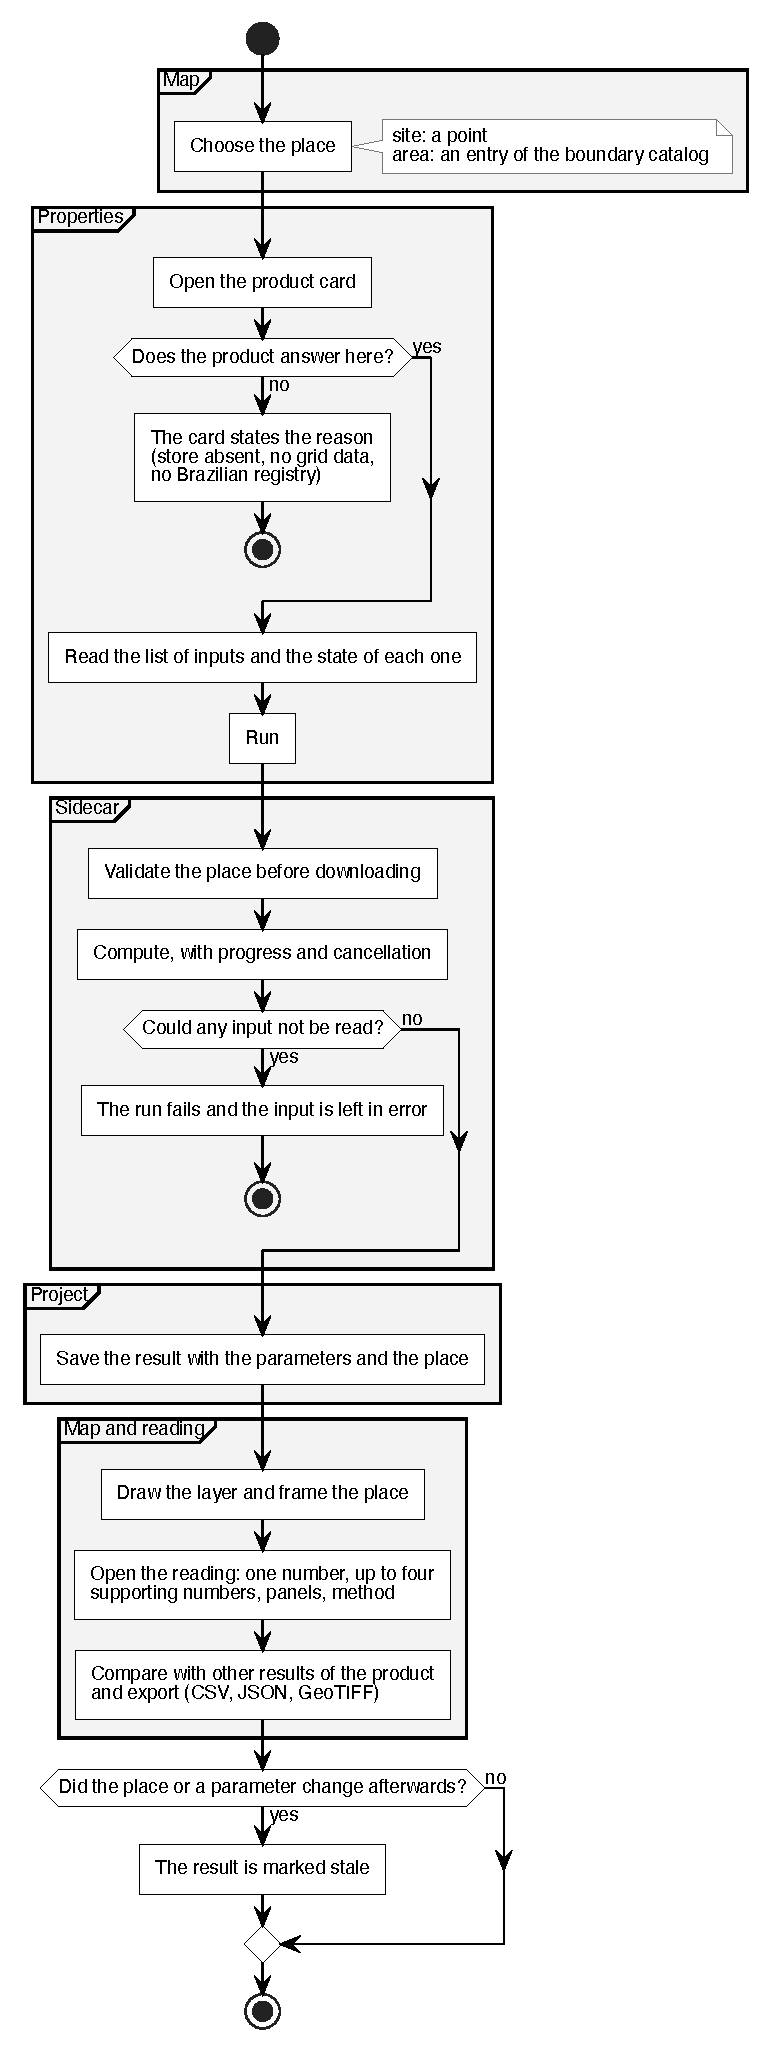
\includegraphics[height=0.86\textheight]{fluxo-leitura-en.pdf}
\caption{The run starts from the place chosen on the map and returns to it
as a layer. Sequence reconstructed from the interface and the sidecar; each
gray band is the part of the application in which the step occurs. The two
side exits end without a result: the product does not answer there, or an
input could not be read.}
\label{fig:fluxo}
\end{figure}

The run is started from the product card in Properties or from the empty
reading, which shows the same list of inputs. The run graph draws the same
inputs as nodes and wires, computed by the same functions, but the run is not
started from it. A wire that enters the run node cannot be cut, and no cut
changes a run. The two wires of the map band, from the region and from the
layer to the map, can be cut: with the cut, the layer is drawn over the whole
footprint of the registry, without the clipping to the region.

\begin{table}[H]
\caption{State of an input in the product card and in the run graph.}
\begin{tabularx}{\linewidth}{l Y}
\toprule
\textbf{State} & \textbf{Meaning} \\
\midrule
not set & the input has no value: no active place, store not connected \\
pending & the value changed after the most recent run \\
reading & a run is in progress \\
read & the most recent run read this value \\
error & the last attempt failed at this input \\
\bottomrule
\end{tabularx}
\end{table}

\begin{figure}[H]
\begin{tabelalarga}
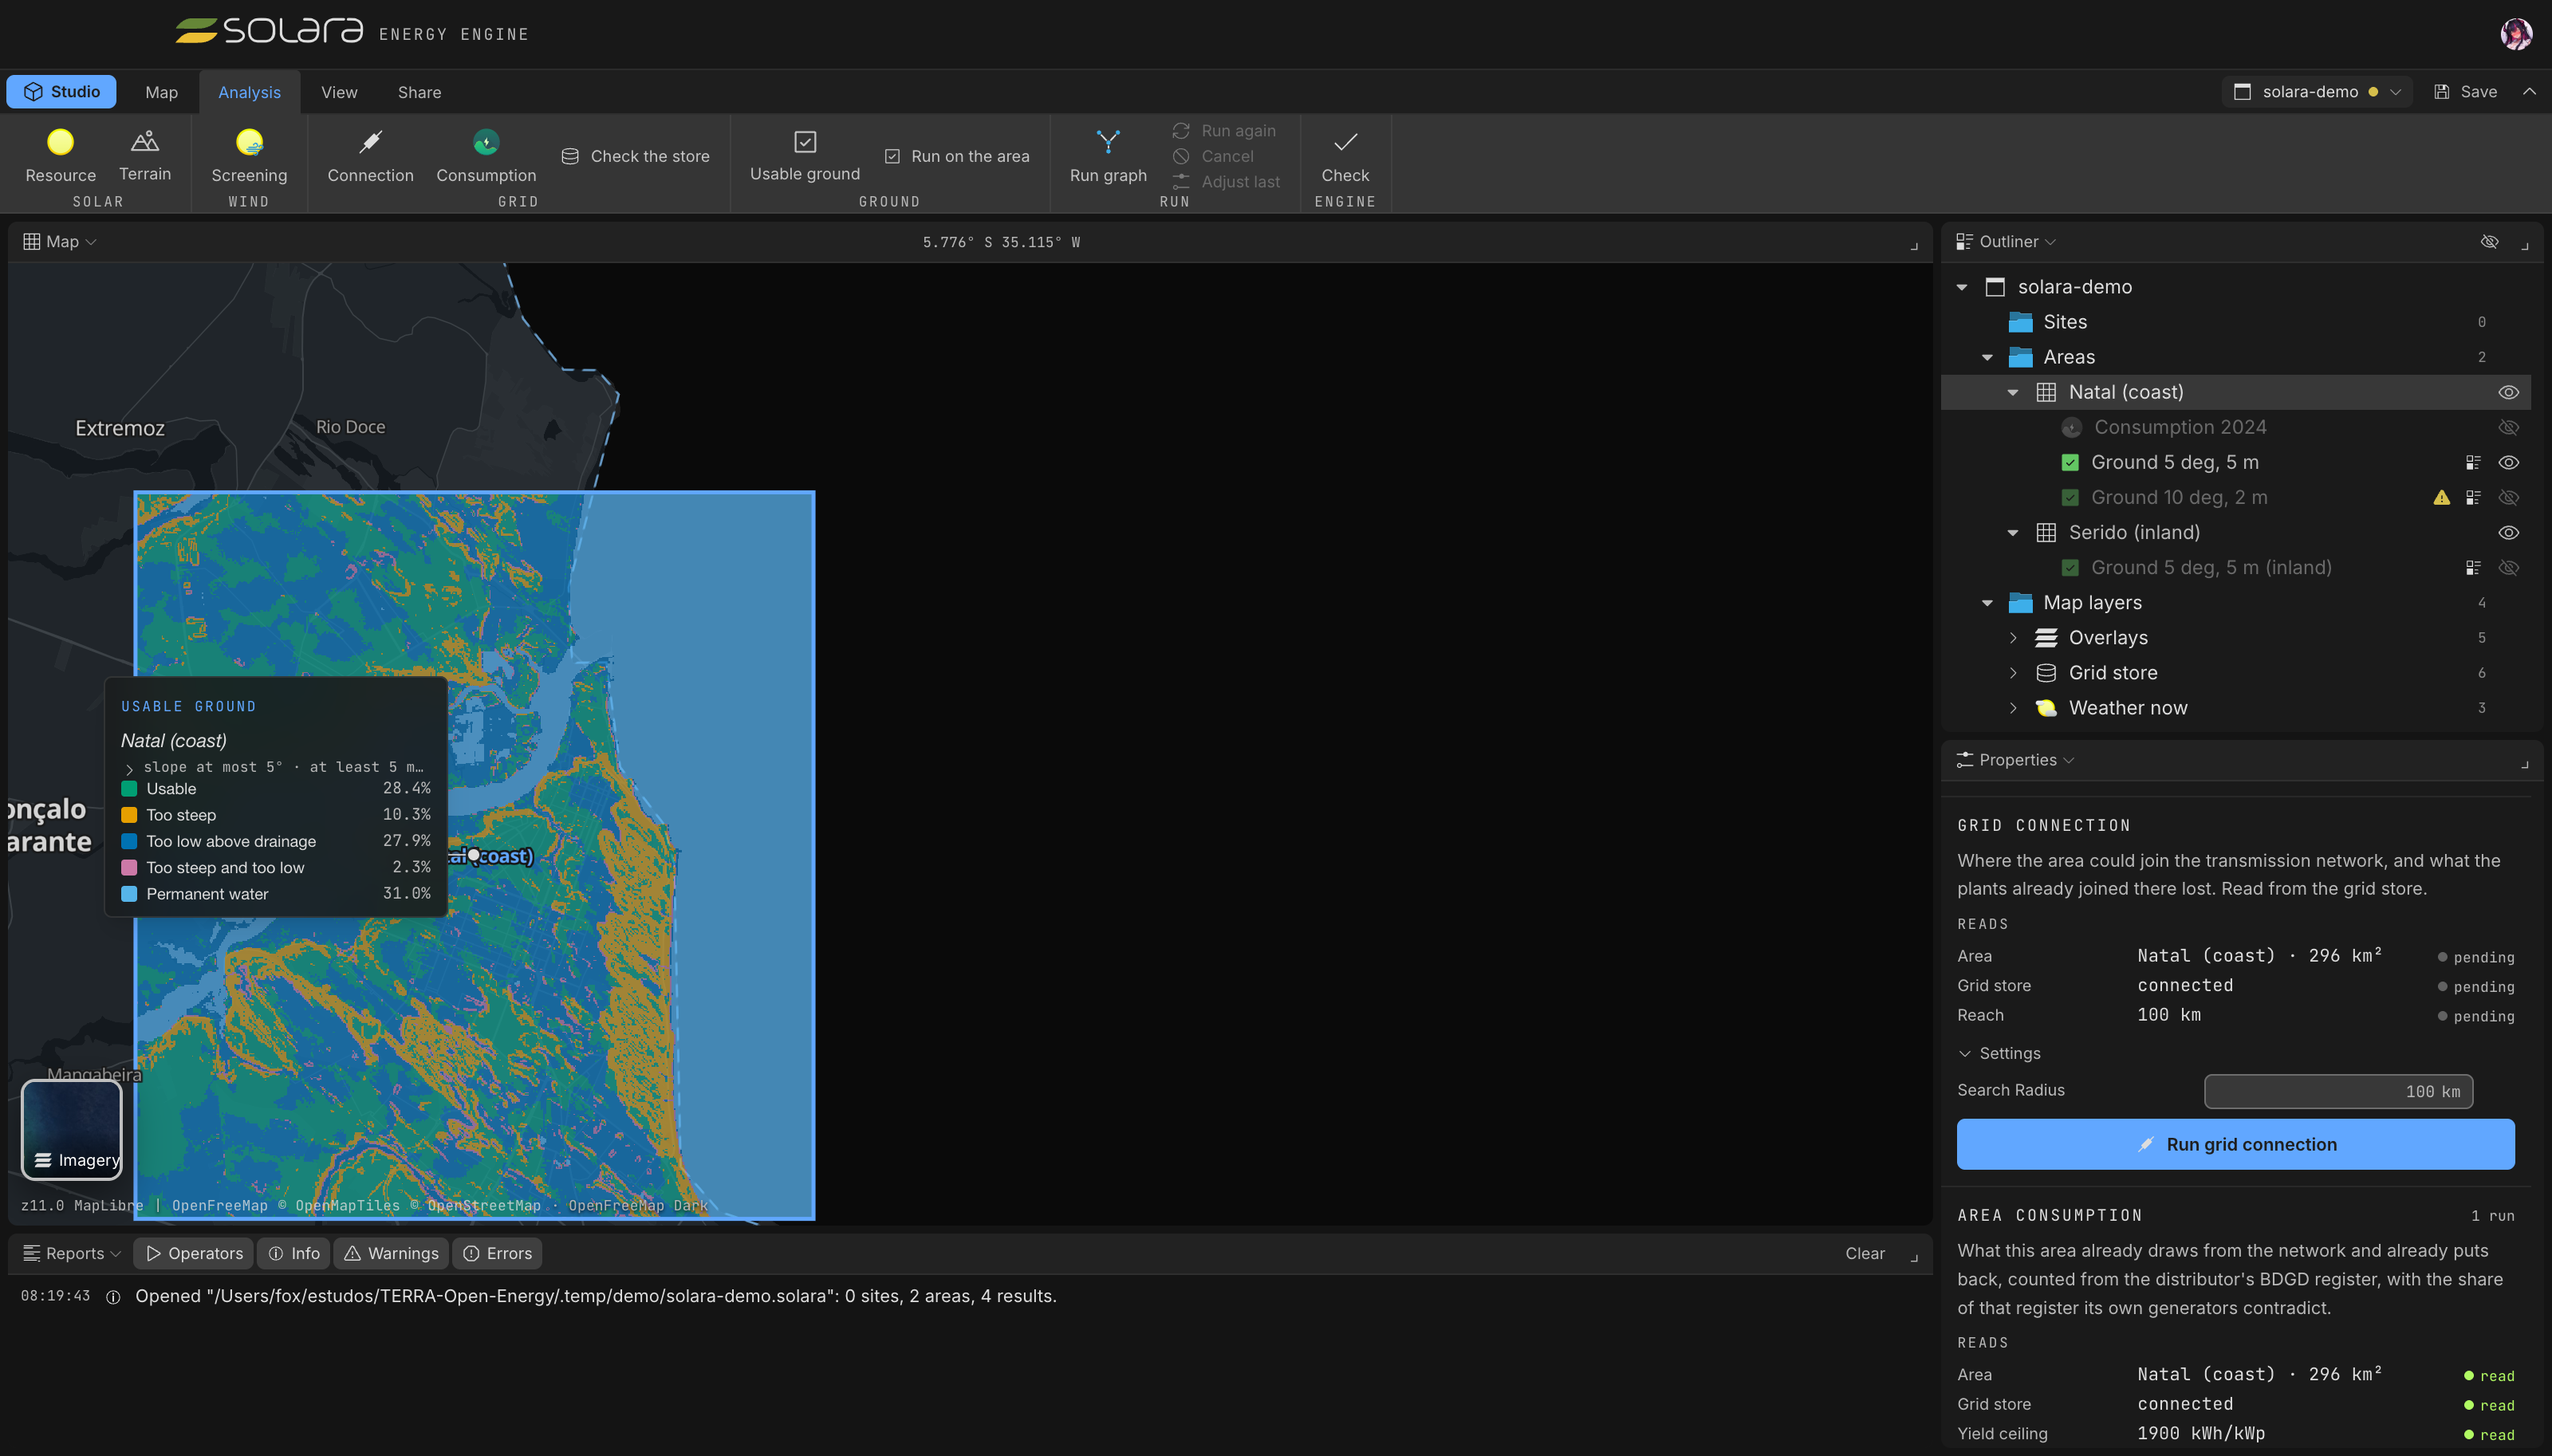
\includegraphics[width=\linewidth]{solara-cartoes-produto.png}
\caption{The product card lists what the run reads and the state of each input before the run. Properties with the area selected: the grid connection card, not yet run, with its three inputs as \enquote{pending}, the search radius parameter and the run button; below it, the area consumption card, already run, with its inputs as \enquote{read}. Screenshot of the demonstration project, like the others in this document; the area \enquote{Natal (coast)} is a four-vertex rectangle saved in the project file, and not a catalog entry.}
\label{fig:cartoes}
\end{tabelalarga}
\end{figure}

\subsection{Layout of a reading}

All readings have the same layout, in this order:

\begin{enumerate}
  \item the product and the status of the result, the number with which the
    product answers, and a line that states where and from what;
  \item up to four supporting numbers, each next to what it is read
    against;
  \item the panel that breaks down the answer, at full width;
  \item the other panels, two per row, or one when the screen area is
    narrow;
  \item how the reading was obtained.
\end{enumerate}

\begin{figure}[H]
\begin{tabelalarga}
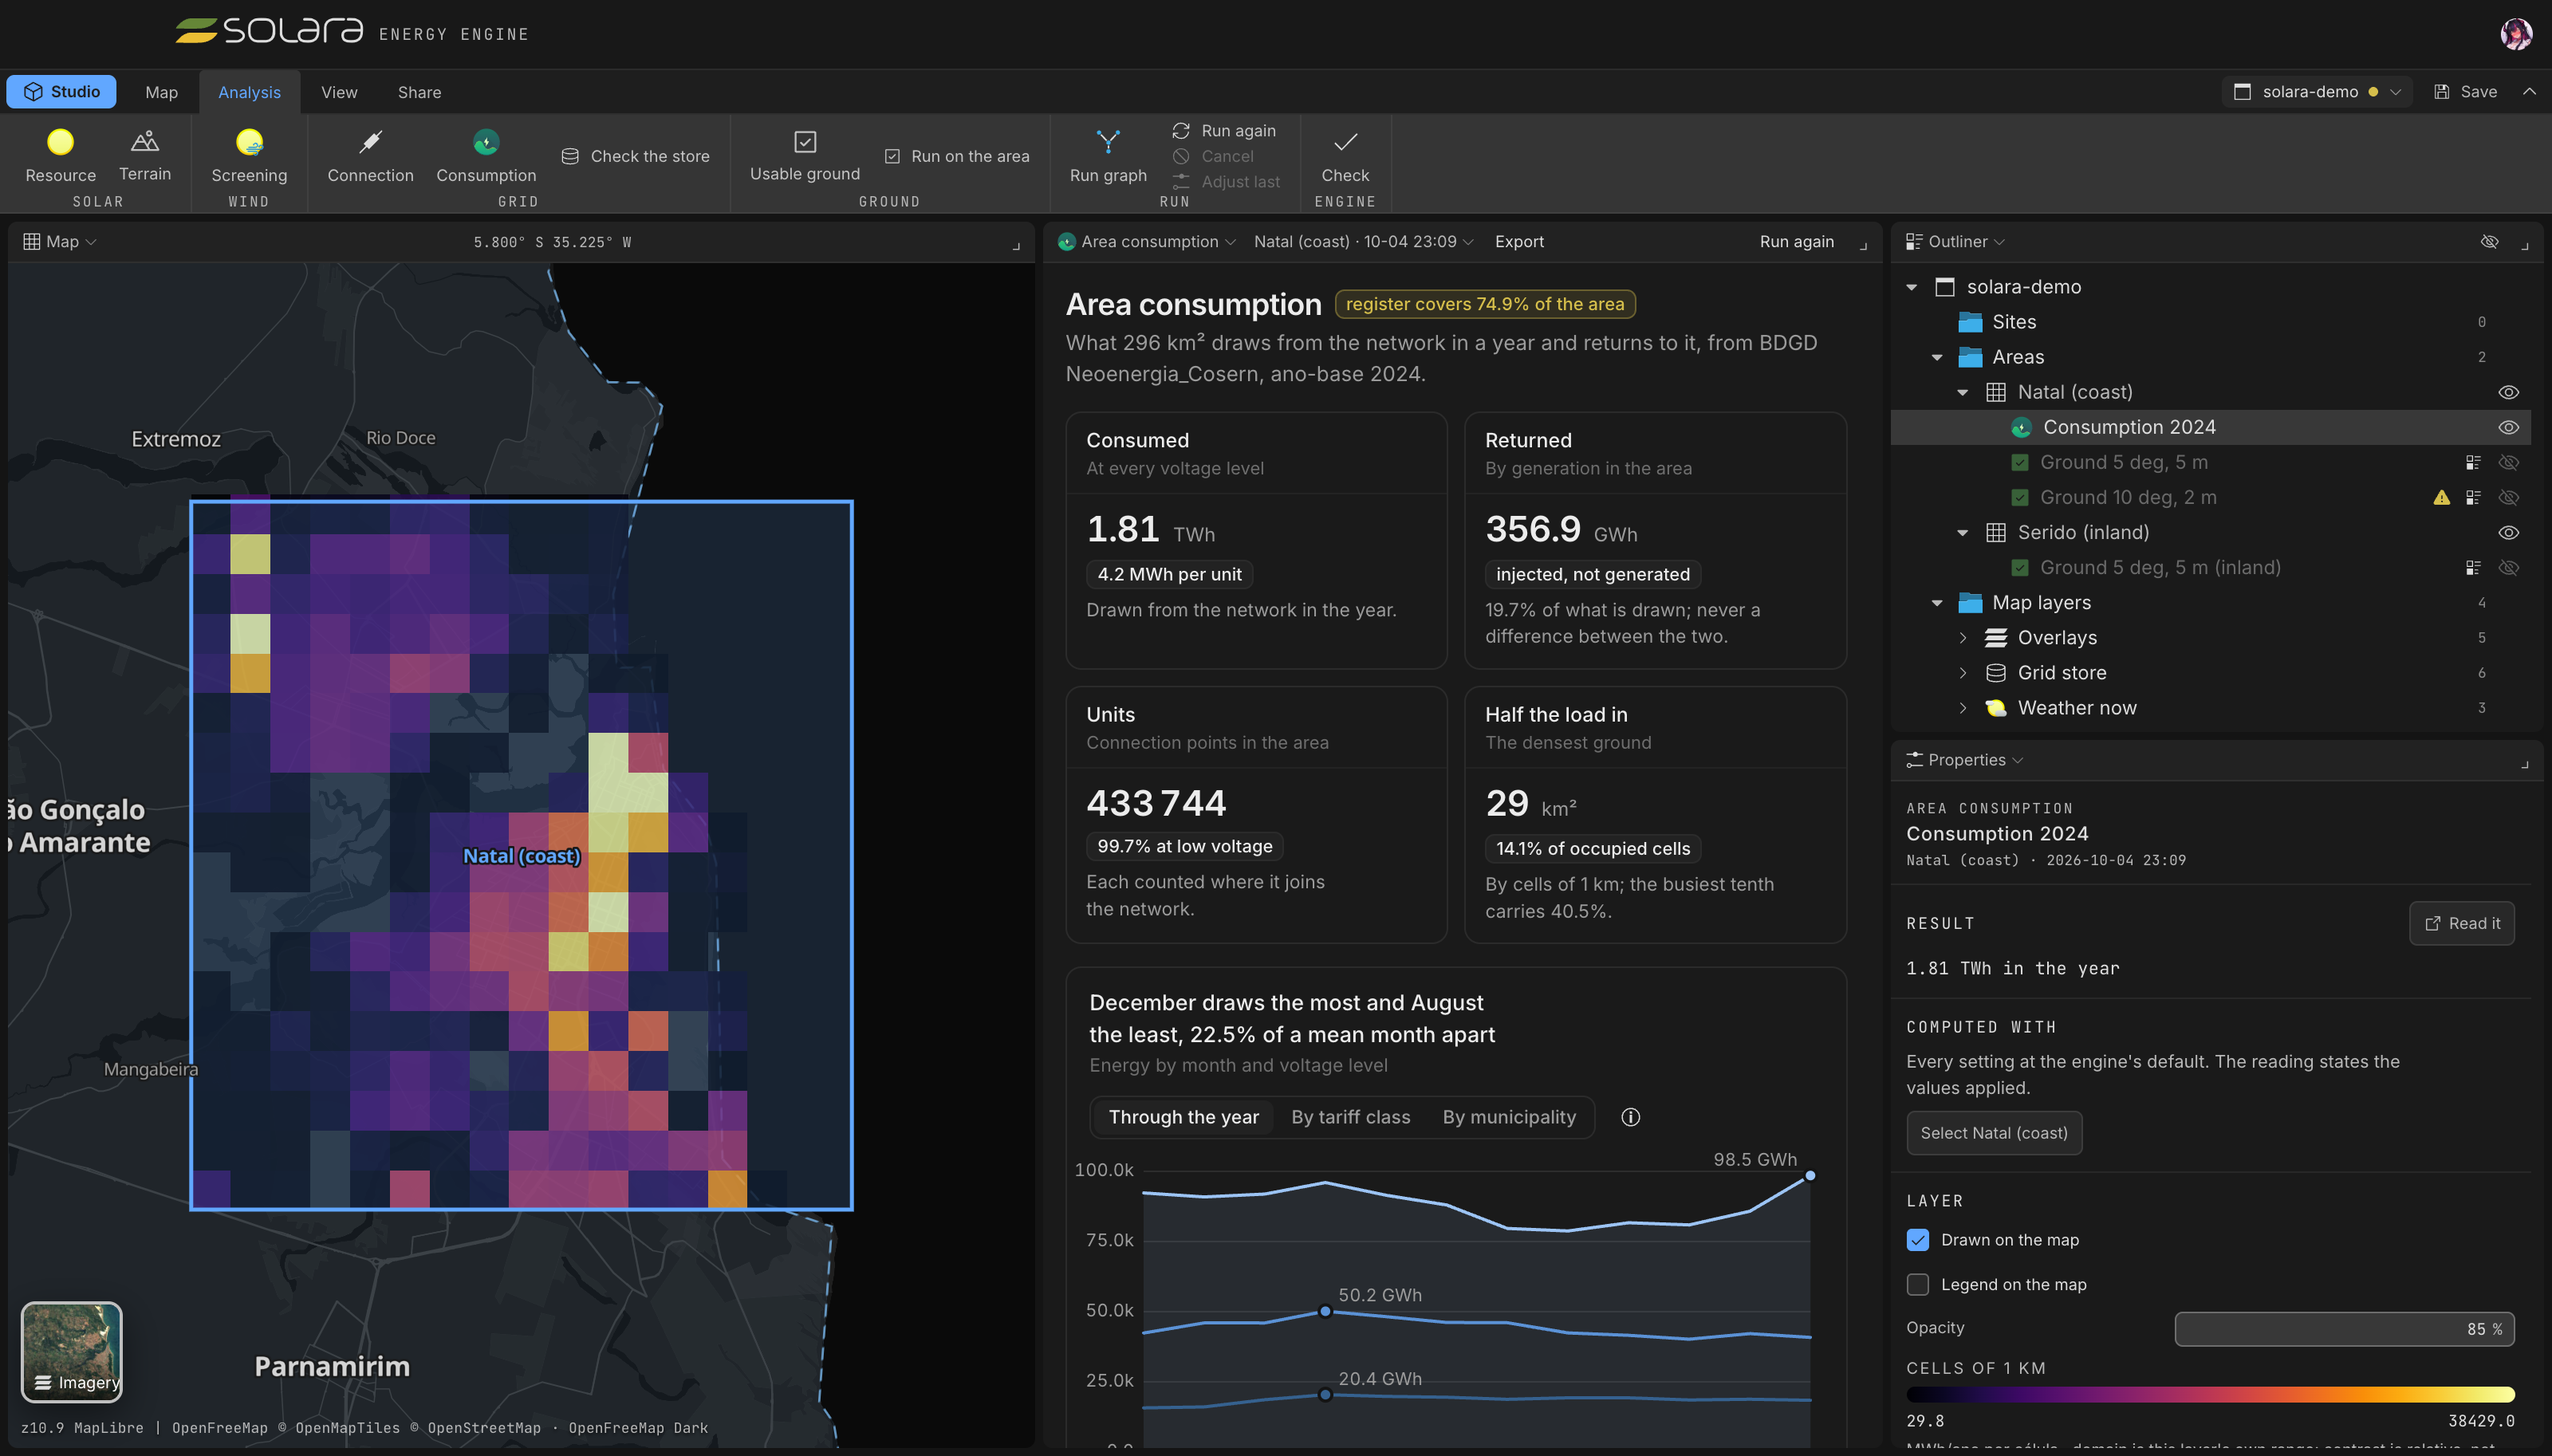
\includegraphics[width=\linewidth]{solara-consumo-area.png}
\caption{The reading opens with one number, four supporting numbers and the panel that breaks down the answer. Area consumption over Natal, BDGD of Neoenergia Cosern, base year 2024: the coverage of the registry next to the title, the injected energy with the qualification \enquote{injected, not generated} next to the number, and the panel of energy by month and voltage level. On the map, the \qty{1}{\kilo\metre} consumption grid. Screenshot of the same demonstration project.}
\label{fig:leitura}
\end{tabelalarga}
\end{figure}

The explanation of a panel is opened by the information button in the header
of the panel. Properties summarizes a result in one line, with the number of
the reading and the button that opens it. Results of the same product are
compared side by side in a table and exported as CSV or JSON. The layer of a
result is also exported as GeoTIFF: the solar terrain layer in
\texttt{float32}, the usable ground layer with the classes. The time of the
computation appears in the reader's time zone on screen, in full UTC in the
JSON and in local time with the offset in the CSV.

\begin{figure}[H]
\begin{tabelalarga}
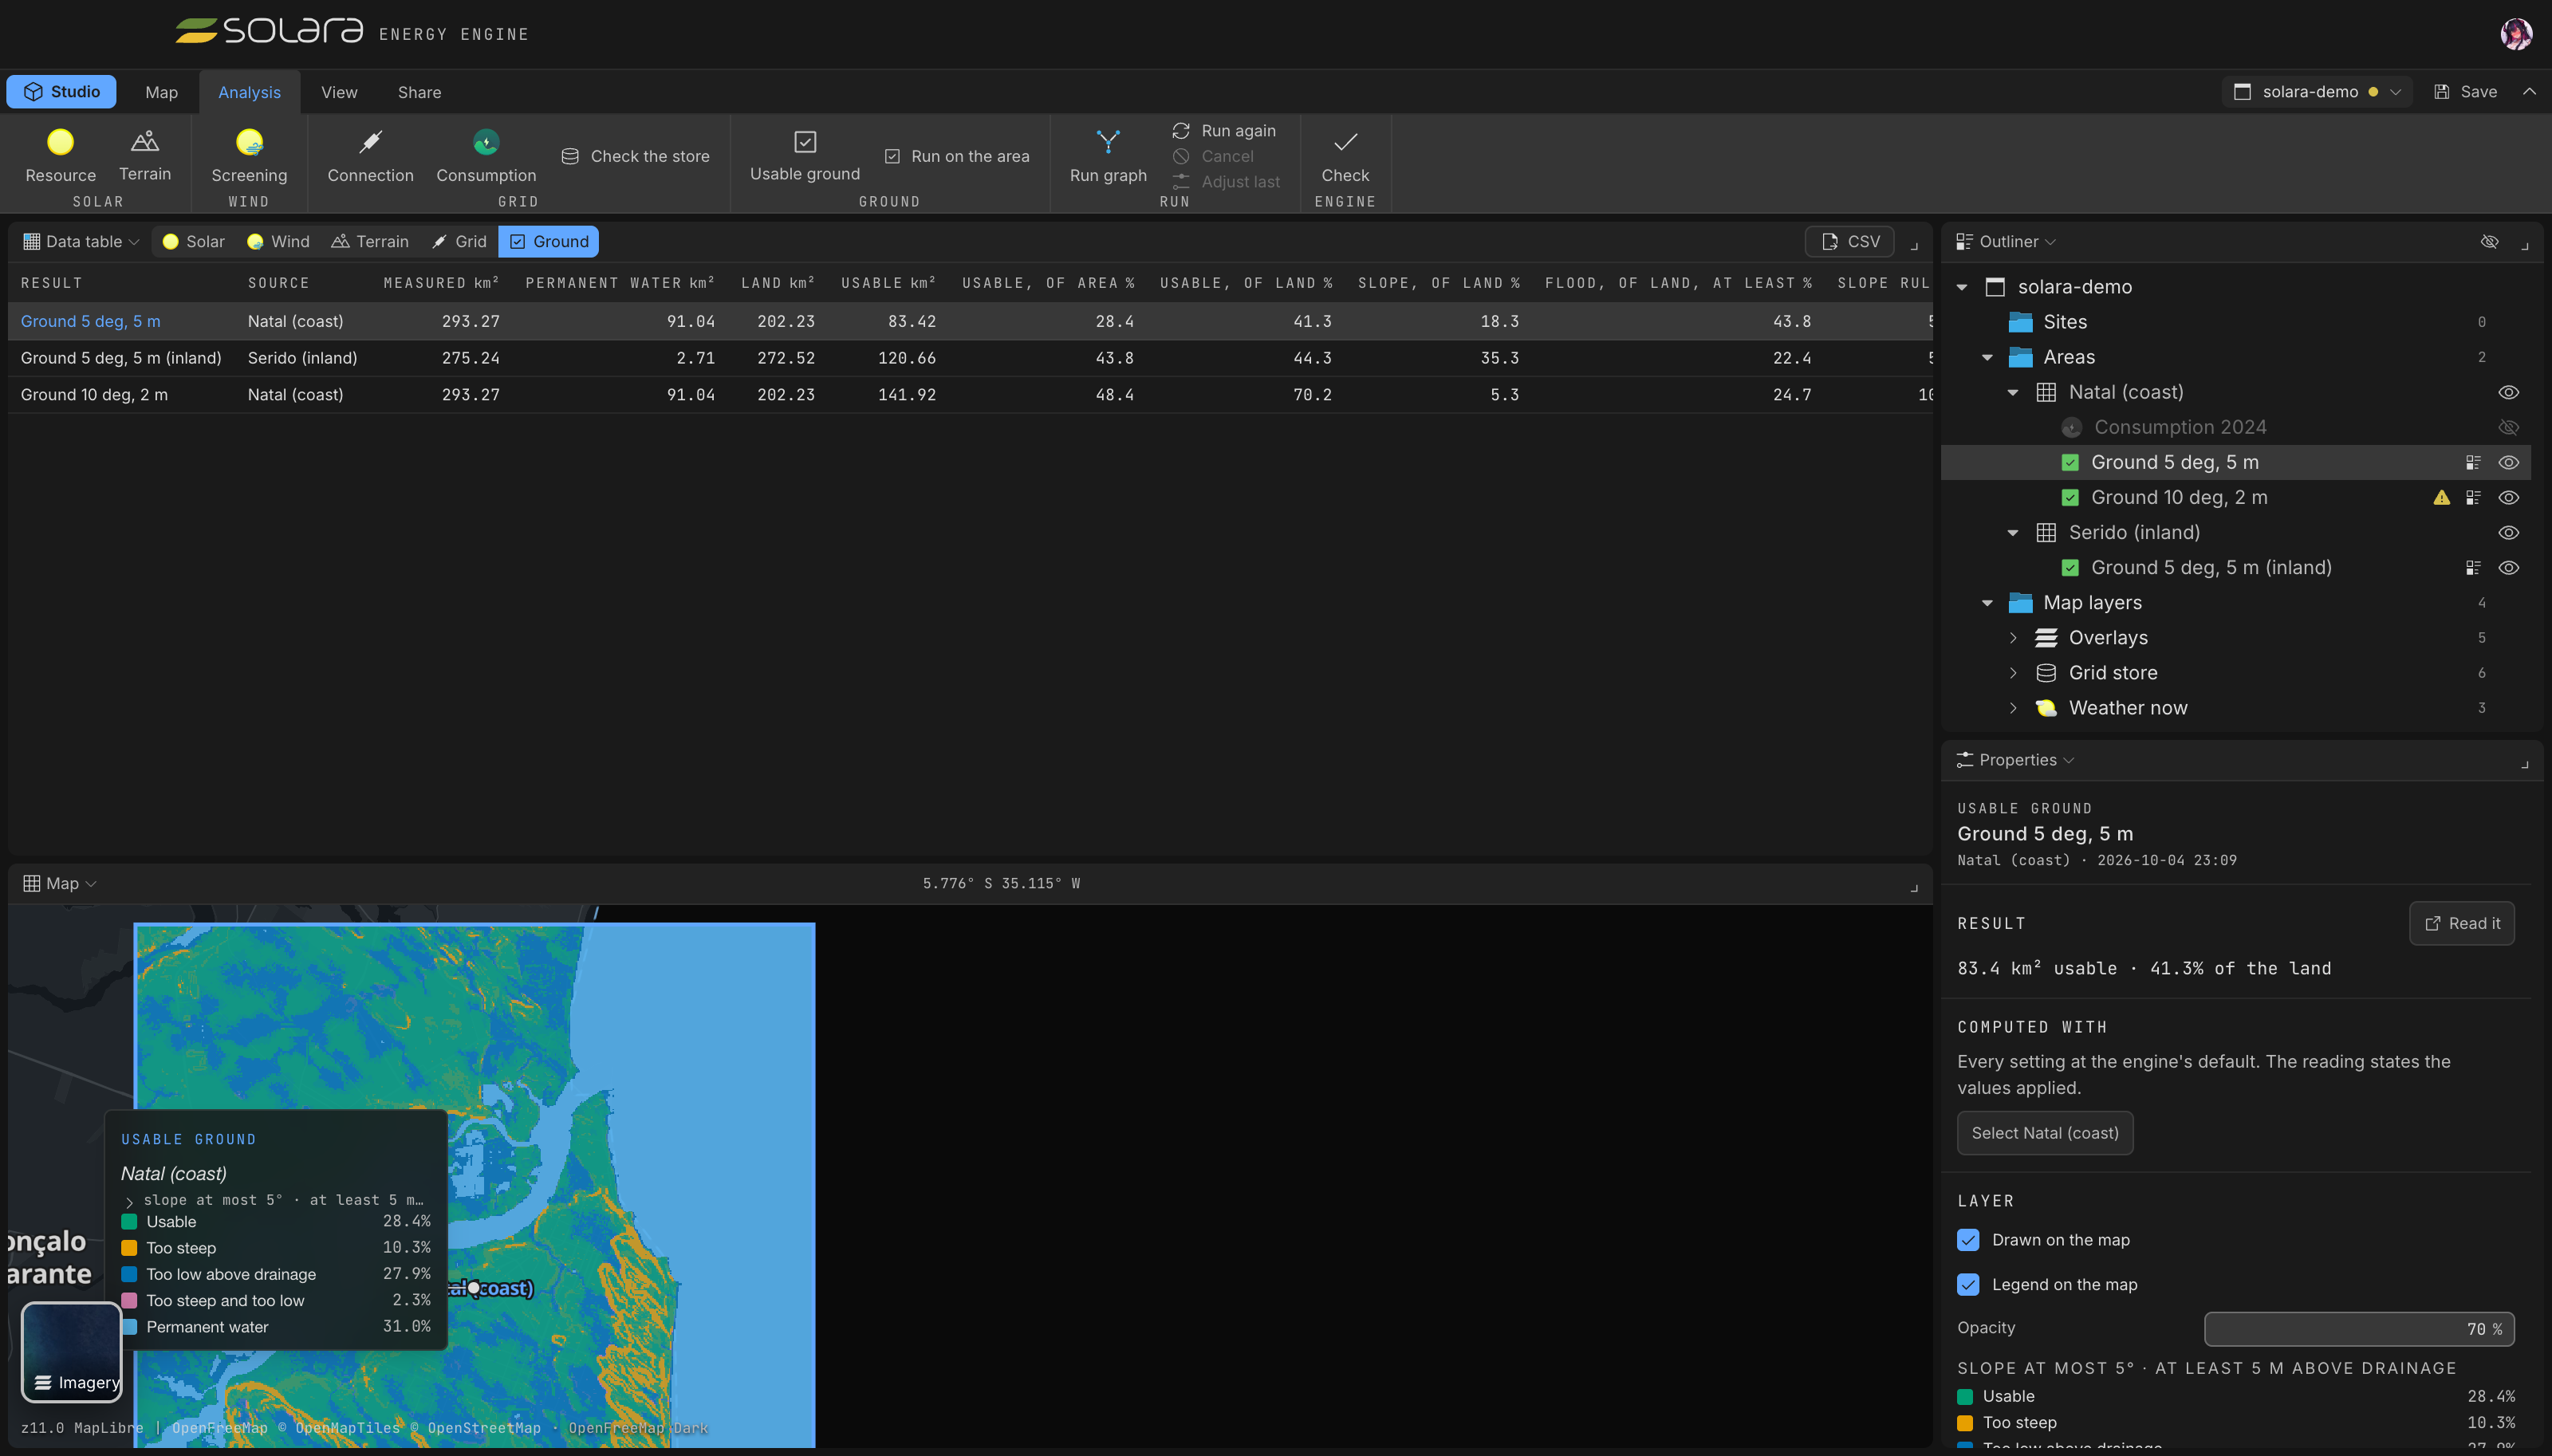
\includegraphics[width=\linewidth]{solara-tabela-comparacao.png}
\caption{Results of the same product are compared row by row. Data table with three usable ground results: two rules over the same coastal area and the default rule over an inland area. Screenshot of the same demonstration project.}
\label{fig:comparacao}
\end{tabelalarga}
\end{figure}

% ===========================================================================
\section{Products}
\label{sec:produtos}
% ===========================================================================

\begin{table}[H]
\begin{tabelalarga}
\caption{The six products, under the names used in the interface.}
\small
\begin{tabularx}{\linewidth}{L{27mm} l Y L{34mm}}
\toprule
\textbf{Product} & \textbf{Read at} & \textbf{What it answers} & \textbf{Source} \\
\midrule
Solar resource & site & global horizontal irradiation by month and by year,
  P10 and P90, optimum tilt, specific yield and capacity factor & NASA POWER,
  pvlib \\
Wind screening & site & wind at hub height, how much it varies with the
  assumed shear, Weibull distribution, density, power curve and wind rose.
  Raw and not validated & NASA POWER (MERRA-2) \\
Solar terrain & area & plane-of-array irradiation on the terrain, at
  \qty{30}{\metre}, with horizon shading, by season & Copernicus DEM GLO-30,
  NASA POWER \\
Grid connection & area & the bus to which the plants of the area are
  connected, the headroom at that bus, what is within reach and how much the
  plants already connected there lost to curtailment & ONS and ANEEL
  registries, in the store \\
Area consumption & area & what the area draws from the grid over the year,
  by voltage level, tariff class and municipality, what distributed
  generation injects, and the distribution on a \qty{1}{\kilo\metre} grid &
  BDGD of the distribution utility, in the store \\
Usable ground & area & how much of the area can hold a plant and what
  excludes the rest, by maximum slope and minimum height above the nearest
  drainage (HAND). Permanent water is removed before the two rules &
  Copernicus DEM GLO-30, ESA WorldCover 2021 \\
\bottomrule
\end{tabularx}
\end{tabelalarga}
\end{table}

\subsection{Conditions of each product}

\begin{itemize}
  \item \textbf{Solar resource, wind screening and solar terrain} read global
    sources and are not blocked by the store.
  \item \textbf{Solar terrain} validates the area before downloading any data
    and limits it to four million cells, about \qtyproduct{55 x 55}{\kilo\metre}.
  \item \textbf{Grid connection} requires a store with lines and substations.
    The reading opens with the bus to which the plants of the area are
    connected, as ONS publishes it, and not with the nearest substation: ONS
    publishes the 500, 230 and \qty{138}{\kilo\volt} buses of a substation at
    the same coordinate, and sorting by distance selects the wrong voltage.
  \item \textbf{Area consumption} requires the Brazilian registry in the
    store and refers to one distribution utility at a time. Before the run,
    the card reports how much of the area the registry covers.
  \item \textbf{Usable ground} applies two rules typed by the user: maximum
    slope, \ang{5} by default, and minimum height above drainage,
    \qty{5}{\metre} by default, where zero turns the rule off. Without the
    water map the run fails. The usable fraction is given twice, of the area
    and of the land within it. Land cover, protected areas and distance to
    the connection are not read.
\end{itemize}

\subsection{Weather at the time of the query}
\label{sec:tempo}

Solara offers four weather readings, each marked as \emph{observed} or
\emph{modeled} and shown with its age. The controls sit on a timeline below
the map.

\begin{table}[H]
\caption{Weather readings. All of them depend on the internet; without it,
each one reports the failure and the rest of the application is not
affected.}
\begin{tabularx}{\linewidth}{l l Y}
\toprule
\textbf{Reading} & \textbf{Kind} & \textbf{Source and cadence} \\
\midrule
Clouds & observed & GOES-East through NASA GIBS, every \qty{10}{\minute},
  true color or infrared, published with a delay of about
  \qty{40}{\minute}; only within the disk of the satellite \\
Rain & observed & RainViewer radar composite, every \qty{10}{\minute}; where
  there is no radar, absence of color is not absence of rain \\
Wind & modeled & GFS at 10 or \qty{100}{\metre}, over the map extent in
  view, as a color field with particles and a label at each place of the
  project \\
Current conditions & modeled & Open-Meteo at a site or area: irradiance,
  cloud, temperature, wind at 10, 80 and \qty{120}{\metre}, the next
  \qty{24}{\hour}, and the comparison with the long-term readings of the
  project \\
\bottomrule
\end{tabularx}
\end{table}

Clouds and rain can be replayed over the last two hours.

% ===========================================================================
\section{Screen}
% ===========================================================================

The window is a studio: the screen is divided into screen areas, each with
an editor, and the arrangements are grouped by subject into workspaces.
Screen areas can be split, joined, resized and maximized, and the arrangement
is kept across restarts.

\begin{figure}[H]
\begin{tabelalarga}
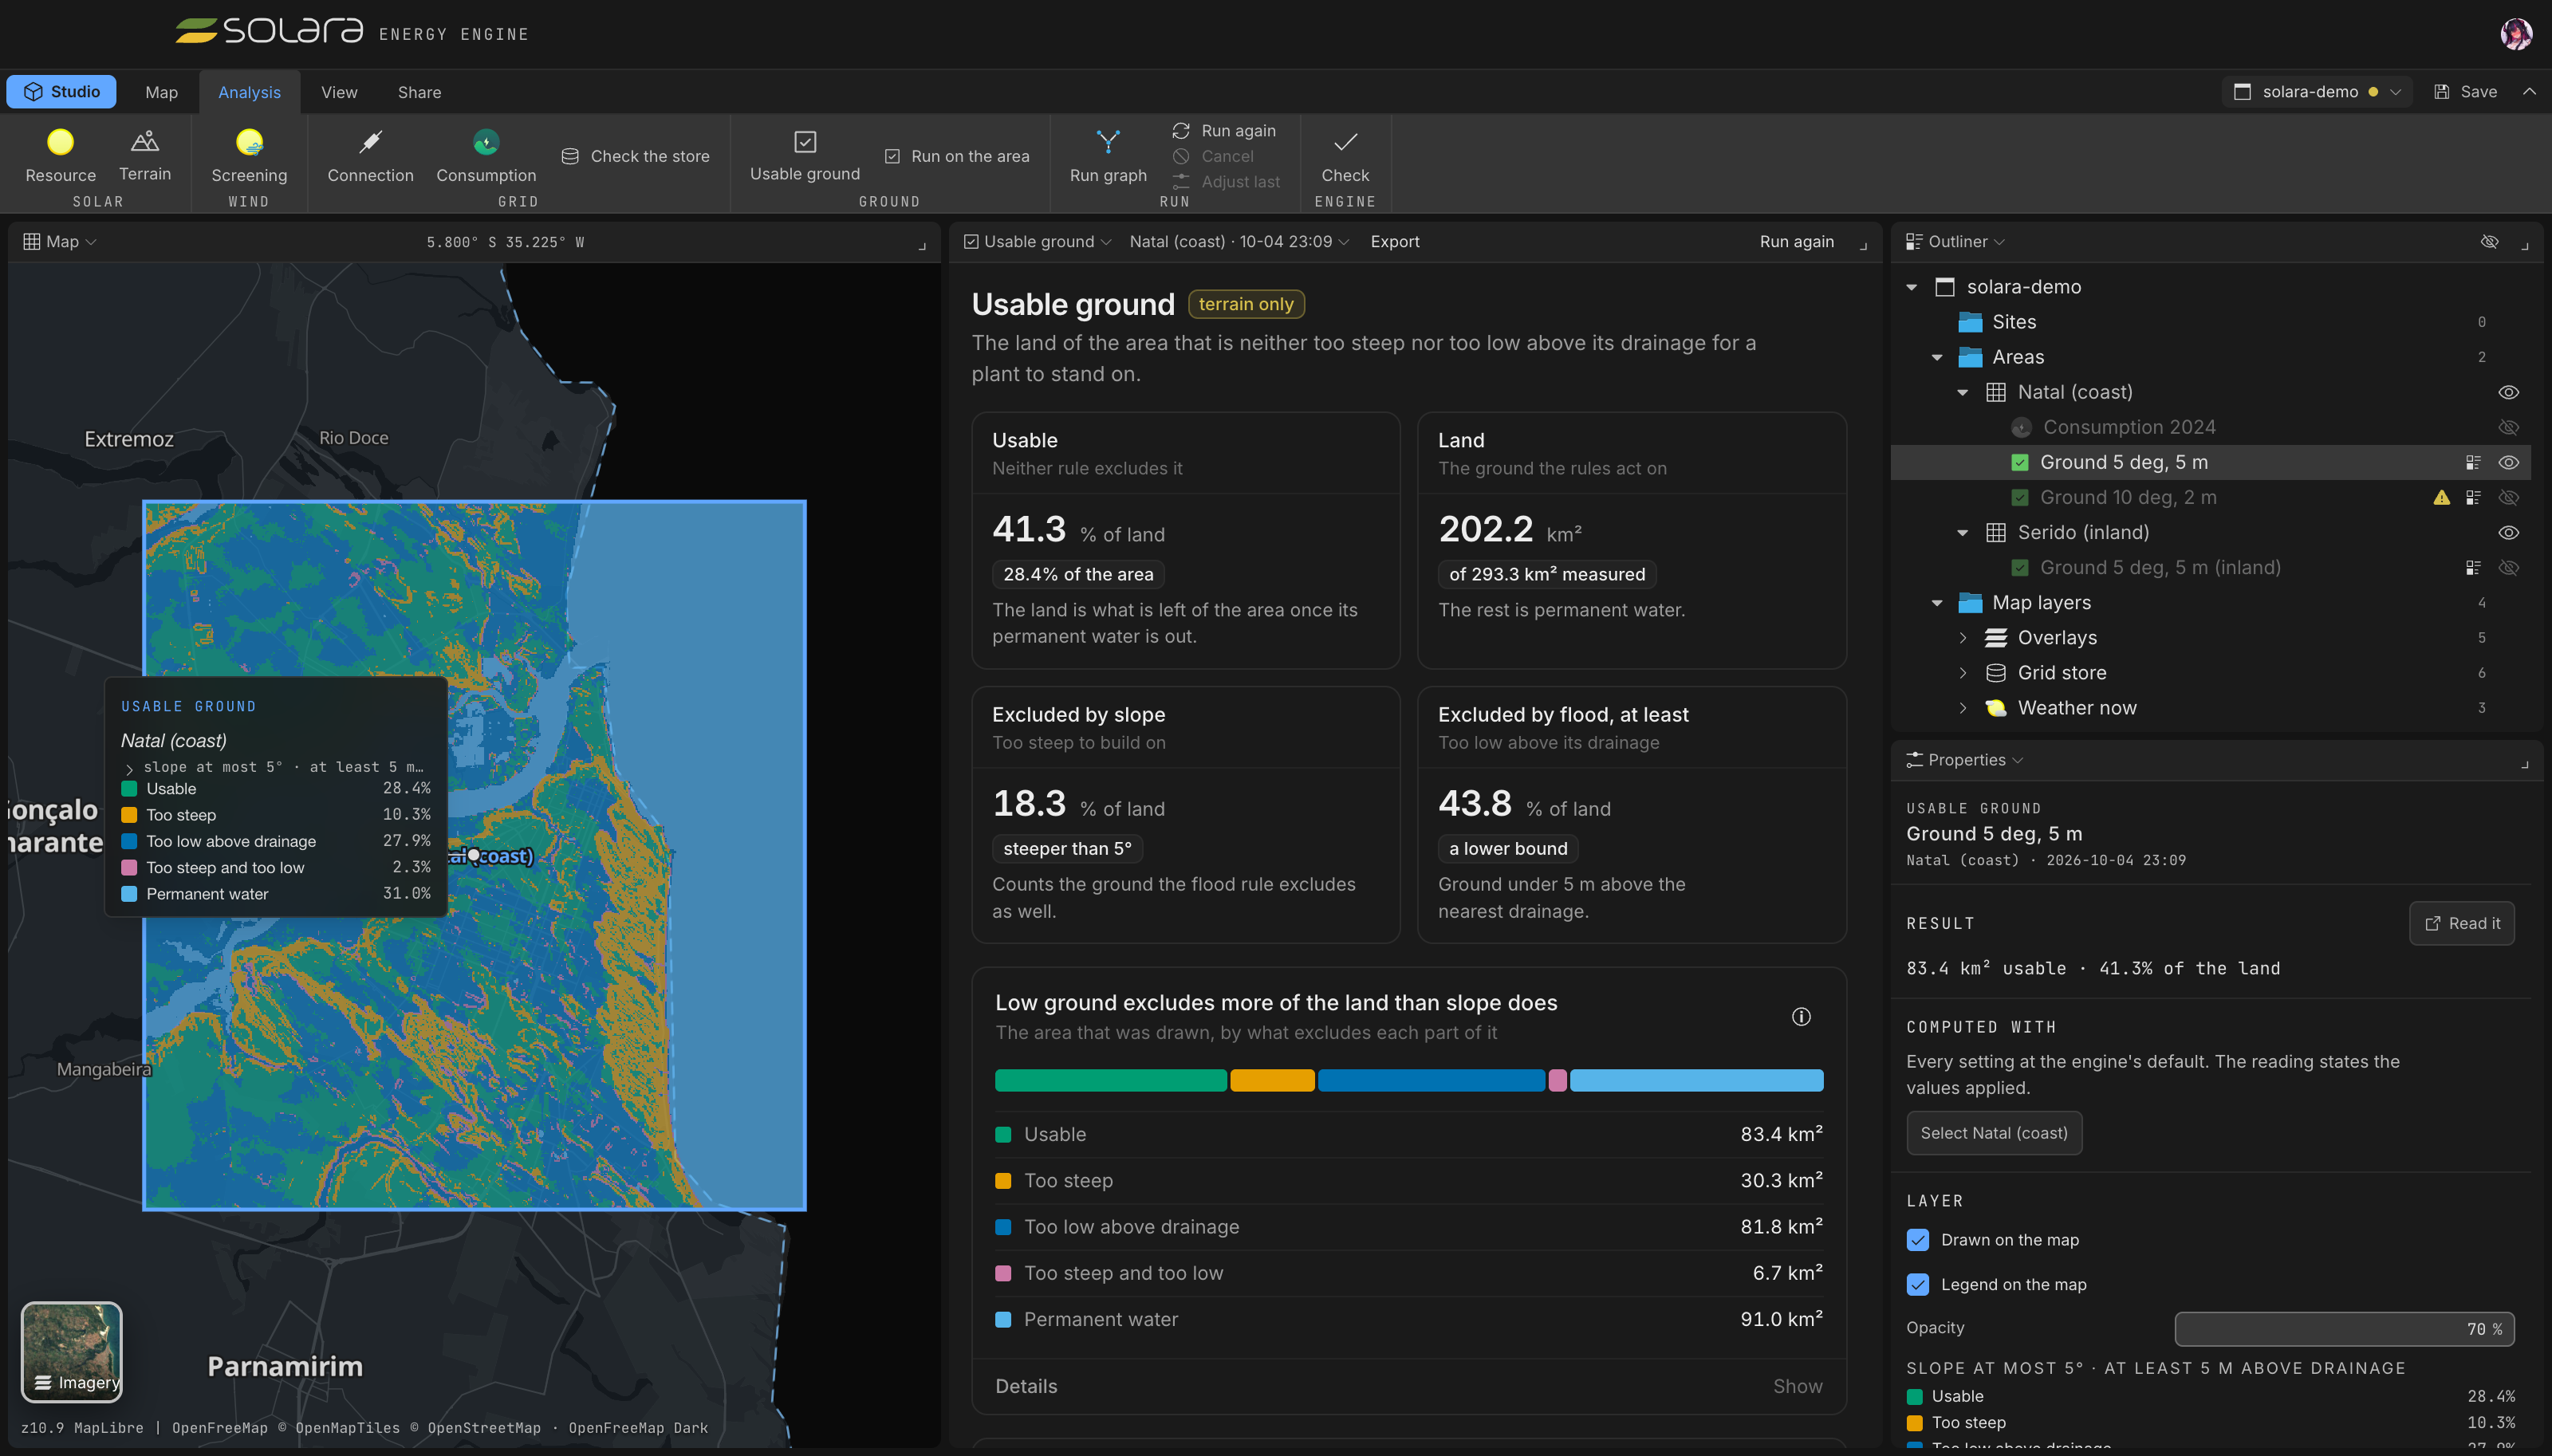
\includegraphics[width=\linewidth]{solara-area-utilizavel.png}
\caption{The map, the reading and the properties of a result sit in the same window. Usable ground over Natal: the class layer on the map with the legend attached to it, the reading in the center with the usable fraction of the land and of the area, and on the right the outliner and Properties with the result in one line. The yellow triangle in the outliner marks a stale result. Screenshot of the same demonstration project.}
\label{fig:tela}
\end{tabelalarga}
\end{figure}

\begin{table}[H]
\caption{Workspace groups.}
\begin{tabularx}{\linewidth}{l l Y}
\toprule
\textbf{Group} & \textbf{Workspaces} & \textbf{Organized around} \\
\midrule
Board & Layout, Graph, Data, Scripting & map, run graph, data table,
  console \\
Solar & Resource, Terrain & solar readings next to the map \\
Wind & Screening & wind reading next to the map \\
Grid & Connection, Demand & connection and consumption readings next to the
  map of plants and lines \\
Ground & Usable ground & usable ground reading next to the map, with the
  class layer \\
\bottomrule
\end{tabularx}
\end{table}

The editors are the map, the outliner, Properties, the run graph, one reading
per product, the data table, the reports and the console.

\subsection{Map layers}

\begin{table}[H]
\caption{Map layers and the condition under which each one is offered.}
\begin{tabularx}{\linewidth}{L{40mm} Y L{38mm}}
\toprule
\textbf{Layer} & \textbf{Content} & \textbf{Offered when} \\
\midrule
Plants in the operational registry & size by capacity & store with the
  Brazilian registry \\
Plants only registered & those that the operational registry does not cover &
  store with plants \\
Lines and buses & lines colored by voltage, in the ANEEL convention &
  store with grid data \\
Footprint of each registry & union of the BDGD sets (\emph{conjuntos}) of
  each distribution utility; on by default & store with the Brazilian
  registry \\
Consumption by municipality & all the municipalities of each registry & store
  with the Brazilian registry \\
SIGEL & wind turbines one by one and strips declared of public utility &
  map over Brazil \\
Night lights & NASA Black Marble, as a check of where there is load &
  always \\
Basemap & dark street map or cloudless Sentinel-2 imagery of 2016, with
  shaded relief under the other layers & always \\
Area result & raster of the solar terrain or of the usable ground classes,
  with legend, visibility and opacity & there is a result in the project \\
\bottomrule
\end{tabularx}
\end{table}

Clicking a feature of a store layer opens a legend at the clicked point. The
SIGEL and night lights layers arrive as images from the services themselves:
they report where something is, not what it is, and cannot be clicked. The
credit in the footer of the map follows the basemap in use and the registries
that are on.

% ===========================================================================
\section{Architecture}
% ===========================================================================

\begin{table}[H]
\caption{Components and the responsibility of each one.}
\begin{tabularx}{\linewidth}{L{36mm} Y}
\toprule
\textbf{Component} & \textbf{Responsibility} \\
\midrule
Interface (webview) & the studio: project state, map, editors, interface
  operators, undo \\
Go/Wails shell & the calls that the interface makes; what each product sends
  and the shape of what comes back; the project file; the results directory
  of the session, served to the interface \\
Python sidecar & the computation. One interpreter per request: the request
  enters as JSON on standard input, the progress leaves on standard error,
  the result leaves as JSON on standard output. One request at a time,
  cancellable \\
Grid store & PostgreSQL with PostGIS on the same machine, read by the
  sidecar \\
Project & a file \texttt{name.solara}, with the terrain rasters in a folder
  \texttt{name.solara-data} next to it \\
\bottomrule
\end{tabularx}
\end{table}

The sidecar protocol is that of TERRA, the program that loads the
\texttt{br} schema of the store, and the actions have the names and the
result shapes of TERRA where the two programs share a product, so that an
action moves from one to the other without change. The raster of a result is
served from the results directory and does not travel as a data URI.

\begin{figure}
\begin{tabelalarga}
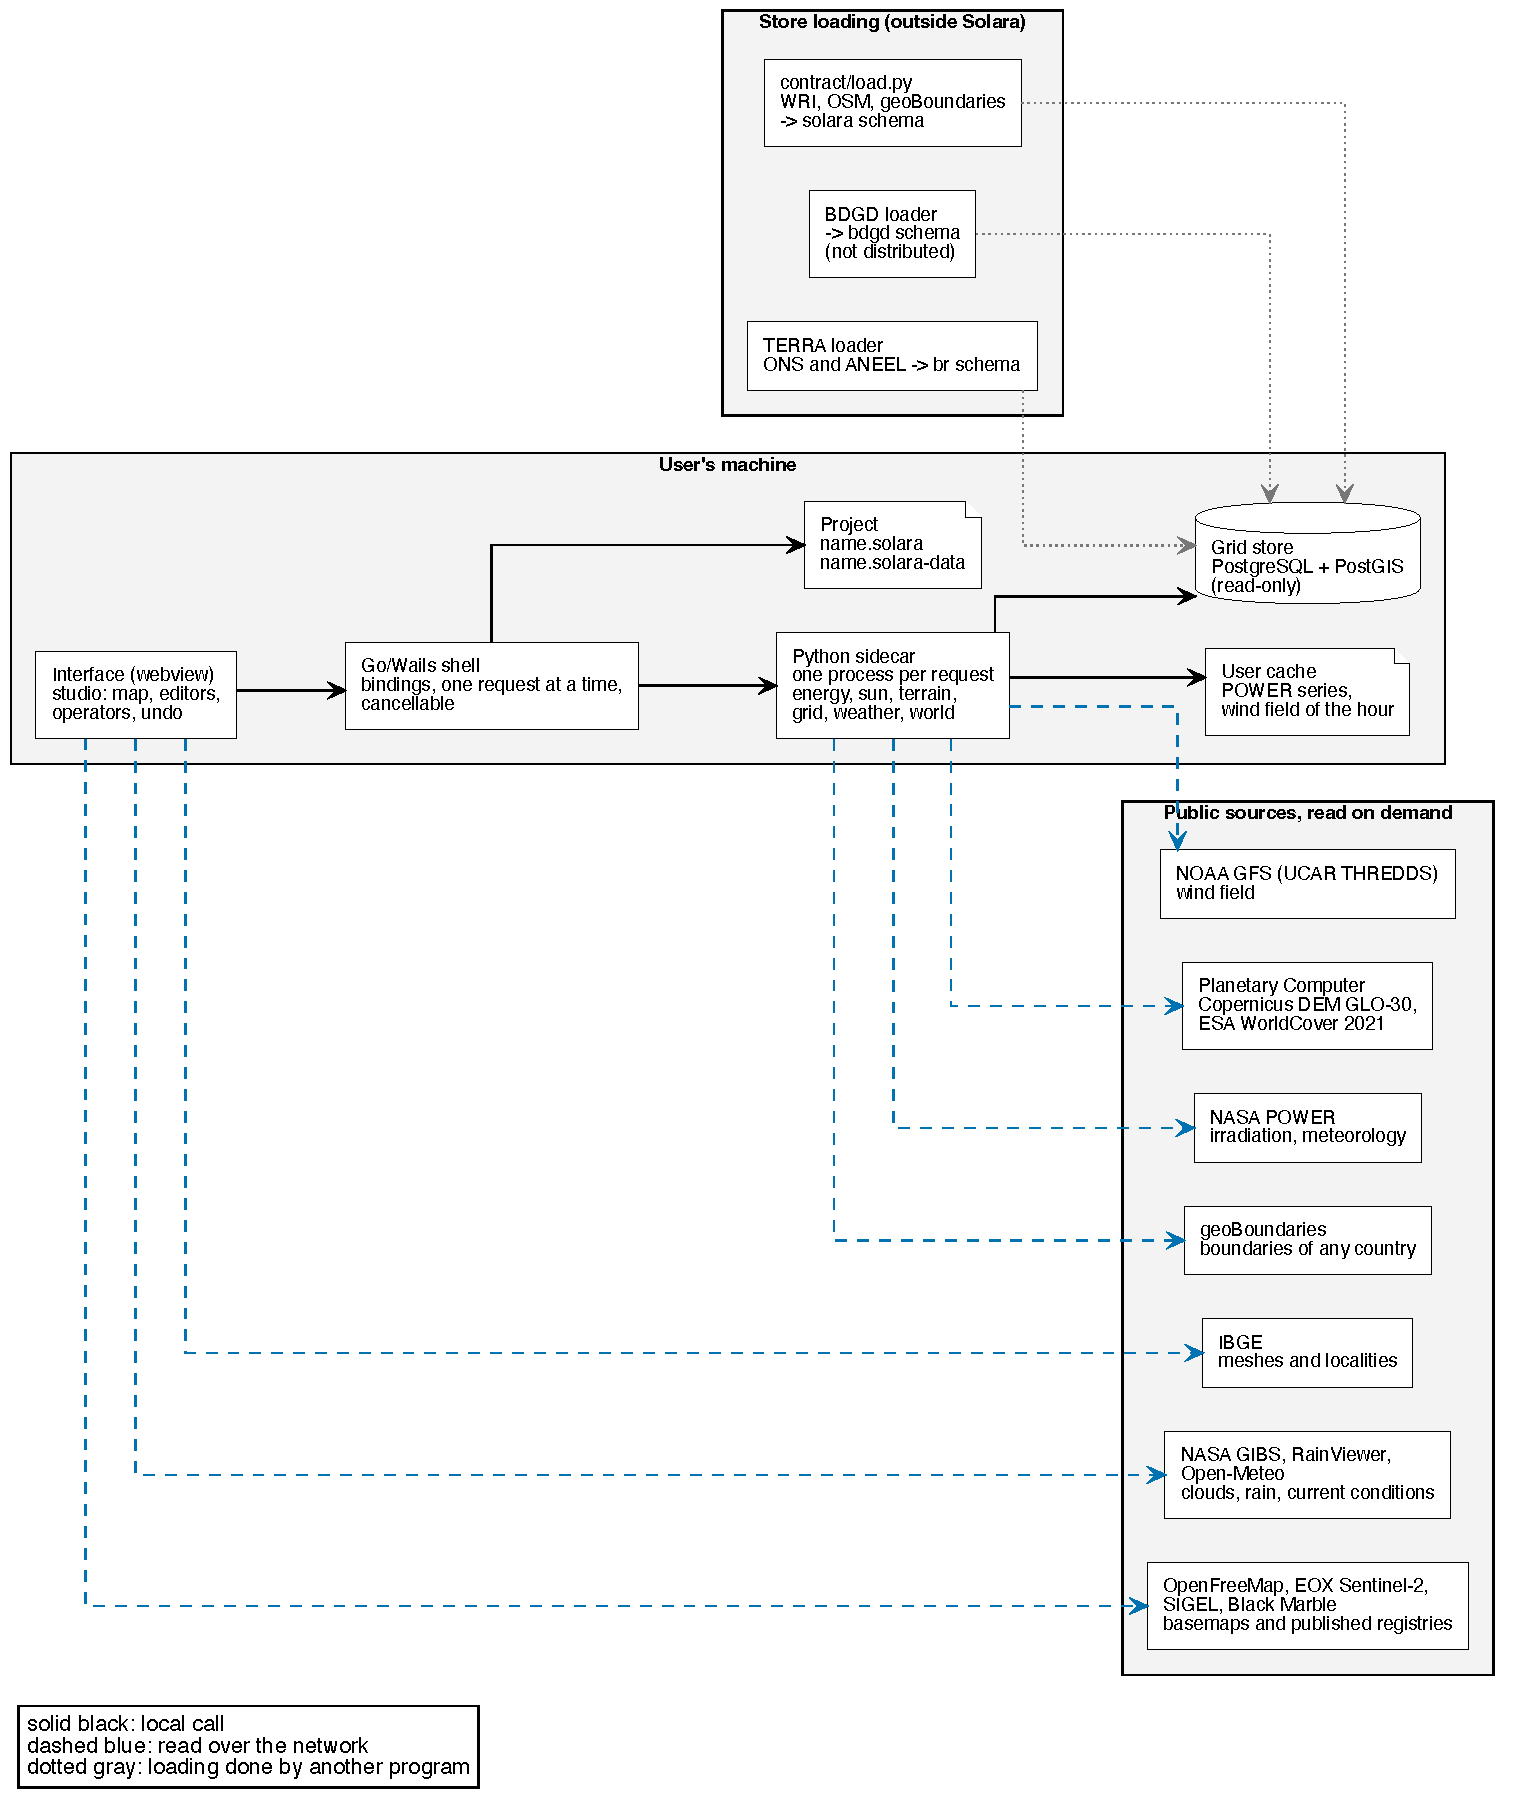
\includegraphics[width=\linewidth]{arquitetura-solara-en.pdf}
\caption{All the computation and all the state stay on the user's machine;
the network supplies only public data. Components surveyed from the Solara
code. Solid black line: local call. Dashed blue line: read over the network.
Dotted gray line: loading of the store done by another program. BDGD: Base de
Dados Geográfica da Distribuidora (geographic database of the distribution
utility). GFS: Global Forecast System. WRI: World Resources Institute. OSM:
OpenStreetMap.}
\label{fig:arquitetura}
\end{tabelalarga}
\end{figure}

\begin{table}[H]
\caption{Where each item is stored.}
\begin{tabularx}{\linewidth}{Y Y}
\toprule
\textbf{What} & \textbf{Where} \\
\midrule
local accounts and the chosen store & user configuration directory \\
NASA POWER series and the wind field of the hour & user cache directory \\
terrain rasters of the session & temporary directory, removed on exit; saved
  with the project \\
studio arrangement, layers that are on, recent files & local storage of the
  webview \\
\bottomrule
\end{tabularx}
\end{table}

% ===========================================================================
\section{Data}
% ===========================================================================

\subsection{Grid store}

The store is a PostgreSQL database with PostGIS. Solara chooses which one to
read in this order: the environment variable \texttt{TERRA\_BR\_DSN}, then
the database connected in the \emph{Grid store} card. Without either of them
there is no store, and every reading that depends on it is refused. The
address \texttt{postgresql:///terra\_br} is what the empty fields of the card
stand for, and it applies only after connecting. TERRA reads the same
variable and, in its absence, uses this address by default. What the store
contains defines what Solara offers.

\begin{table}[H]
\caption{Schemas of the store and what each one enables.}
\begin{tabularx}{\linewidth}{l Y Y}
\toprule
\textbf{Schema} & \textbf{Content} & \textbf{Enables} \\
\midrule
\texttt{br} & ANEEL plant register, ONS transmission registry and the ONS
  registry of curtailment of photovoltaic plants; loaded by TERRA & plant,
  line and bus layers; grid connection with curtailment \\
\texttt{bdgd} & consumer units and distributed generators with month-by-month
  energy, and the sets of each distribution utility, by base year & area
  consumption; footprint of each registry; consumption by municipality \\
\texttt{solara} & contract version~1: plants, substations, lines and
  boundaries of any country & plant and grid layers; grid connection; area
  catalog \\
\bottomrule
\end{tabularx}
\end{table}

The contract fixes the units (MW, kV, MVA) and the projection (EPSG:4326);
the conversion is up to whoever prepares the store. An unknown value is null,
not zero. The line declares whether the geometry follows the route of the
conductor or is the straight segment between the ends; the distance to a
straight segment is a lower bound, and the reading reports this. Curtailment,
consumption by distribution utility, concession areas and time series are not
in the contract.

\subsection{Sources}

\begin{table}[H]
\begin{tabelalarga}
\caption{Data sources and terms of use.}
\small
\begin{tabularx}{\linewidth}{L{42mm} Y L{52mm}}
\toprule
\textbf{Data} & \textbf{Source} & \textbf{Terms} \\
\midrule
Irradiation and meteorology & NASA POWER & public \\
Elevation & Copernicus DEM GLO-30, through the Microsoft Planetary Computer &
  free, with attribution \\
Permanent water & ESA WorldCover 2021 v200, \qty{10}{\metre}, through the
  Planetary Computer & CC BY 4.0 \\
Plant register & ANEEL (SIGA) & open data \\
Transmission and curtailment & ONS & open data \\
Consumption and distributed generation & BDGD, ANEEL & open data \\
Administrative boundaries & IBGE; geoBoundaries & open data; CC BY 4.0 \\
Clouds & NOAA GOES-East, through NASA GIBS & public \\
Rain & RainViewer & free, with attribution; requests limited per address \\
Wind field & NOAA GFS, through UCAR THREDDS & public; research service with
  no availability guarantee \\
Current conditions & Open-Meteo & CC BY 4.0; free for non-commercial use \\
Street basemap & OpenFreeMap, OpenStreetMap & ODbL \\
Imagery basemap & EOX Sentinel-2 cloudless 2016 & CC BY 4.0; from 2017
  onwards, CC BY-NC-SA \\
\bottomrule
\end{tabularx}
\end{tabelalarga}
\end{table}

% ===========================================================================
\section{Standing caveats}
\label{sec:ressalvas}
% ===========================================================================

The caveats in this section apply to the current readings. They reproduce
what the sources state, and are not defects to be fixed.

\begin{itemize}
  \item \textbf{Distributed generation in the BDGD is injection, not
    generation.} The registry carries what passed through the meter of the
    distribution utility; self-consumption does not pass through it. For
    Cosern, base year 2024, the median generator reports \qty{51}{\percent}
    of the yield modeled by solar resource at the same place. The quantity
    serves a grid question and not a generation question. The definition is
    not confirmed in the regulation: the requests for the annex of REN
    956/2021 and for the BDGD manual received no response.
  \item \textbf{The installed capacity column mixes units.} Some rows are in
    kW and some in W. The reading treats values above 75 as W, which is a
    heuristic and does not cover all cases; the reading that reports
    installed capacity states that it normalized the values.
  \item \textbf{The municipality is the floor of an area.}
  \item \textbf{The footprint of a registry is not a concession area.} It is
    the union of the sets of the registry and answers where the registry has
    data, not who holds the concession.
  \item \textbf{The exclusion by height above drainage, in usable ground, is
    a lower bound.} The elevation model is read over the area and a margin
    of 2 to \qty{5}{\kilo\metre}, not over the upstream basin. A channel that
    enters from outside the margin arrives without its contributing area,
    and less ground is excluded than would otherwise be. The number appears
    as \enquote{at least}.
  \item \textbf{The water in usable ground is the permanent water mapped in
    2021.} Seasonal water, rivers narrower than a few cells, wetlands and
    whatever changed since then remain subject to the two rules. The sea is
    counted as ground where the map has no data.
  \item \textbf{Wind screening is raw and not validated.}
  \item \textbf{The connection reading is not a grid access opinion
    (\emph{parecer de acesso}).}
\end{itemize}

% ===========================================================================
\section{Evolution}
\label{sec:evolucao}
% ===========================================================================

The two tables reproduce the Solara work list reported by the owner on
2026-10-05. The list is not in a Solara file, and the column \enquote{What it
already has} was not checked against the code. A \emph{workstream} is a
subject of the list; it can cover part of a product of
section~\ref{sec:produtos} or more than one. Solar terrain has no item in the
list.

\begin{table}[H]
\begin{tabelalarga}
\caption{Workstreams that already exist and what is missing in each one.}
\small
\begin{tabularx}{\linewidth}{L{27mm} L{27mm} Y Y}
\toprule
\textbf{Workstream} & \textbf{Current product} & \textbf{What it already has} & \textbf{What is missing} \\
\midrule
Ground screening & Usable ground & slope, flooding and permanent water &
  land cover, mangrove and wetland, protected areas, largest contiguous
  usable block \\
Solar resource & Solar resource & irradiation at a point from reanalysis &
  satellite source, ready-made maps \\
Photovoltaic generation & Solar resource & reference array of
  \qty{1}{\kilo\wattpeak}, losses as a single ratio & module and inverter
  library, detailed losses, horizon at the point \\
Wind resource & Wind screening & screening at a point with reanalysis at
  \qty{10}{\metre} and \qty{50}{\metre} & a better source at hub height,
  mapped relief and roughness, import of mast measurements \\
Wind generation & Wind screening & one fixed turbine, raw values & turbine
  catalog, turbine layout, wake, long-term correction \\
Grid & Grid connection & lines, substations, point of connection, headroom
  and curtailment, Brazil only & connection queue, power flow, grids of other
  countries \\
Consumption & Area consumption & monthly consumption of an area from the
  BDGD & hourly load curve of a customer, tariff values \\
\bottomrule
\end{tabularx}
\end{tabelalarga}
\end{table}

\begin{table}[H]
\caption{Workstreams that do not exist and what each one depends on.
\enquote{Chaining} is the use of the result of one product as an input of
another.}
\begin{tabularx}{\linewidth}{L{48mm} Y}
\toprule
\textbf{Workstream} & \textbf{Depends on} \\
\midrule
Financial & photovoltaic or wind generation, and chaining between results \\
Storage and hybrids & generation, price series and chaining \\
Market and revenue & price source per country \\
Environmental impact (wind) & turbine layout \\
Land and permitting & land tenure base per country \\
System planning & grid and consumption; it is close to a separate program \\
\bottomrule
\end{tabularx}
\end{table}

% ===========================================================================
\section{Open questions}
\label{sec:abertas}
% ===========================================================================

\begin{enumerate}
  \item \textbf{Target customer.} Solara serves those who study sites and
    areas for generation. The distribution-utility track of the feature
    catalog depends on private data and on a continuous service, which are
    outside the stated scope. It remains to be decided whether this track is
    dropped, postponed or treated as a separate product.
  \item \textbf{Forecasting models.} No Solara product reads a forecasting
    model from the experiments of the project. It remains to be defined
    whether any of them becomes a product and at which scale of place.
  \item \textbf{BDGD loader.} Area consumption depends on the \texttt{bdgd}
    schema, and the program that loads it is not part of Solara. Until it
    is, the product is reproducible only on a machine that already has the
    store.
  \item \textbf{Commercial use.} The current conditions reading uses the
    free tier of Open-Meteo, restricted to non-commercial use, and the
    imagery basemap is restricted to the 2016 edition, because the editions
    from 2017 onwards carry a non-commercial license.
  \item \textbf{Area below the municipality.} No source subdivides a
    municipality; neighborhoods and census tracts are not reading areas.
\end{enumerate}

\end{document}
